%%%%%%%%%%%%%%%% VRb2J
\begin{figure}[h]
  \centering
    \subfigure[]{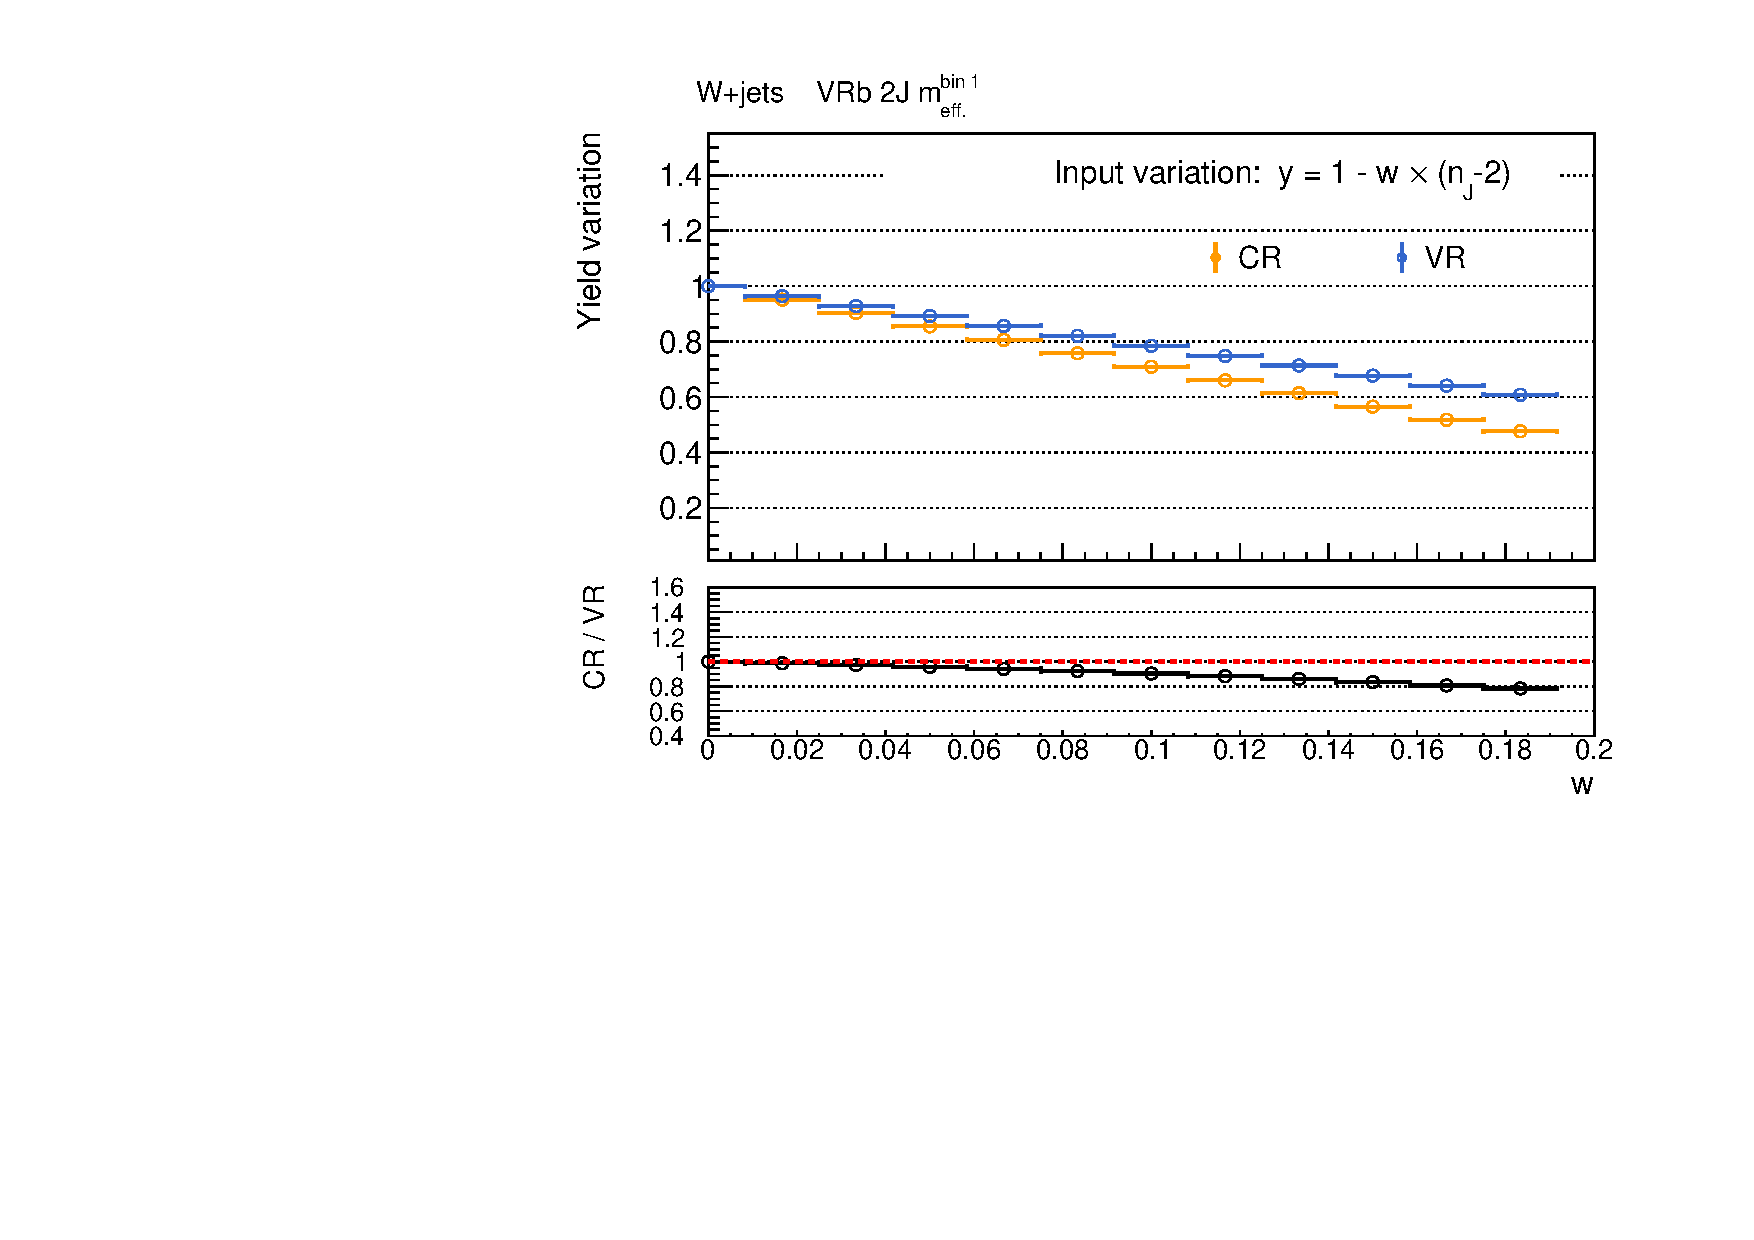
\includegraphics[width=0.488\textwidth]{figures/BGestimation/valid_extp/SFTF_wjets_VRb2JMEFF1_extp_var2J__nJet30.pdf}}
    \subfigure[]{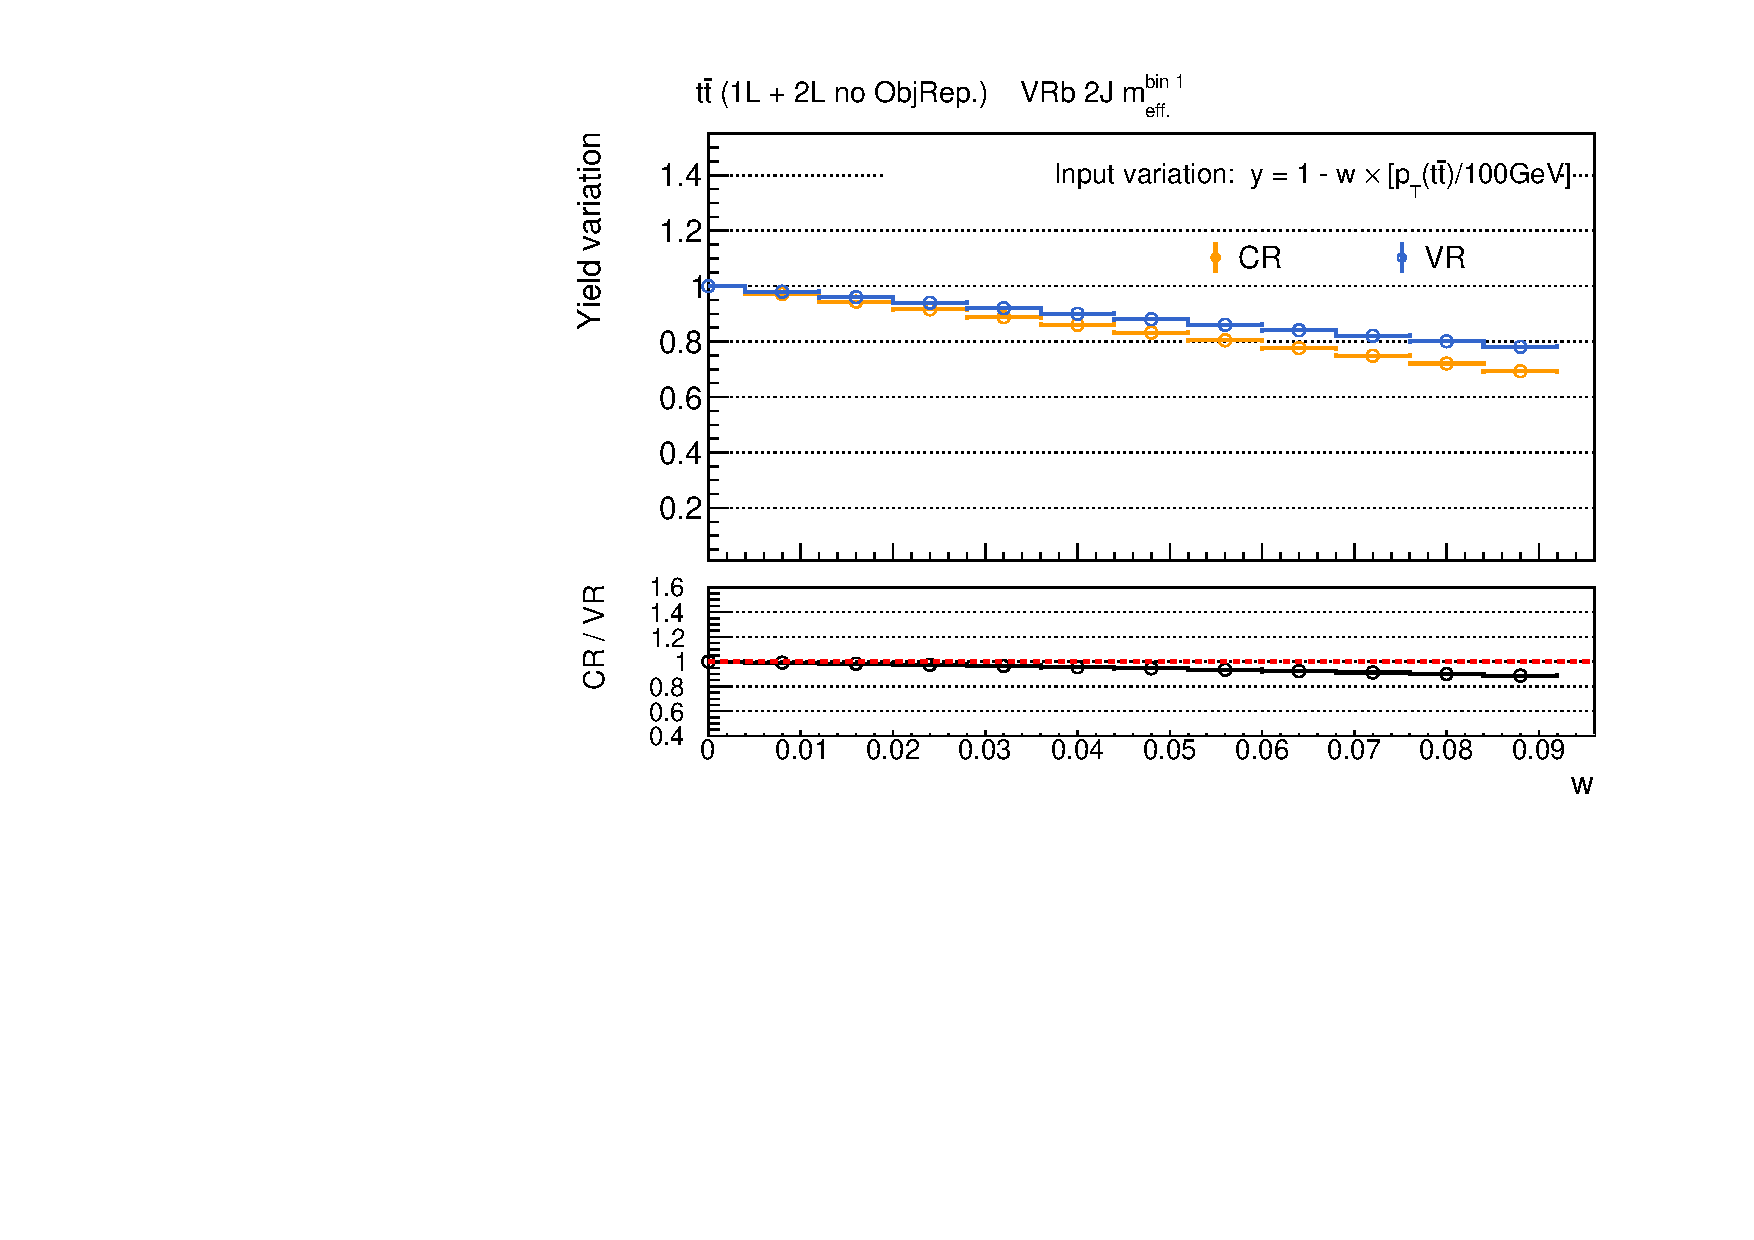
\includegraphics[width=0.488\textwidth]{figures/BGestimation/valid_extp/SFTF_ttNoObjRep_VRb2JMEFF1_extp_var2J__ttPt.pdf}}
    \subfigure[]{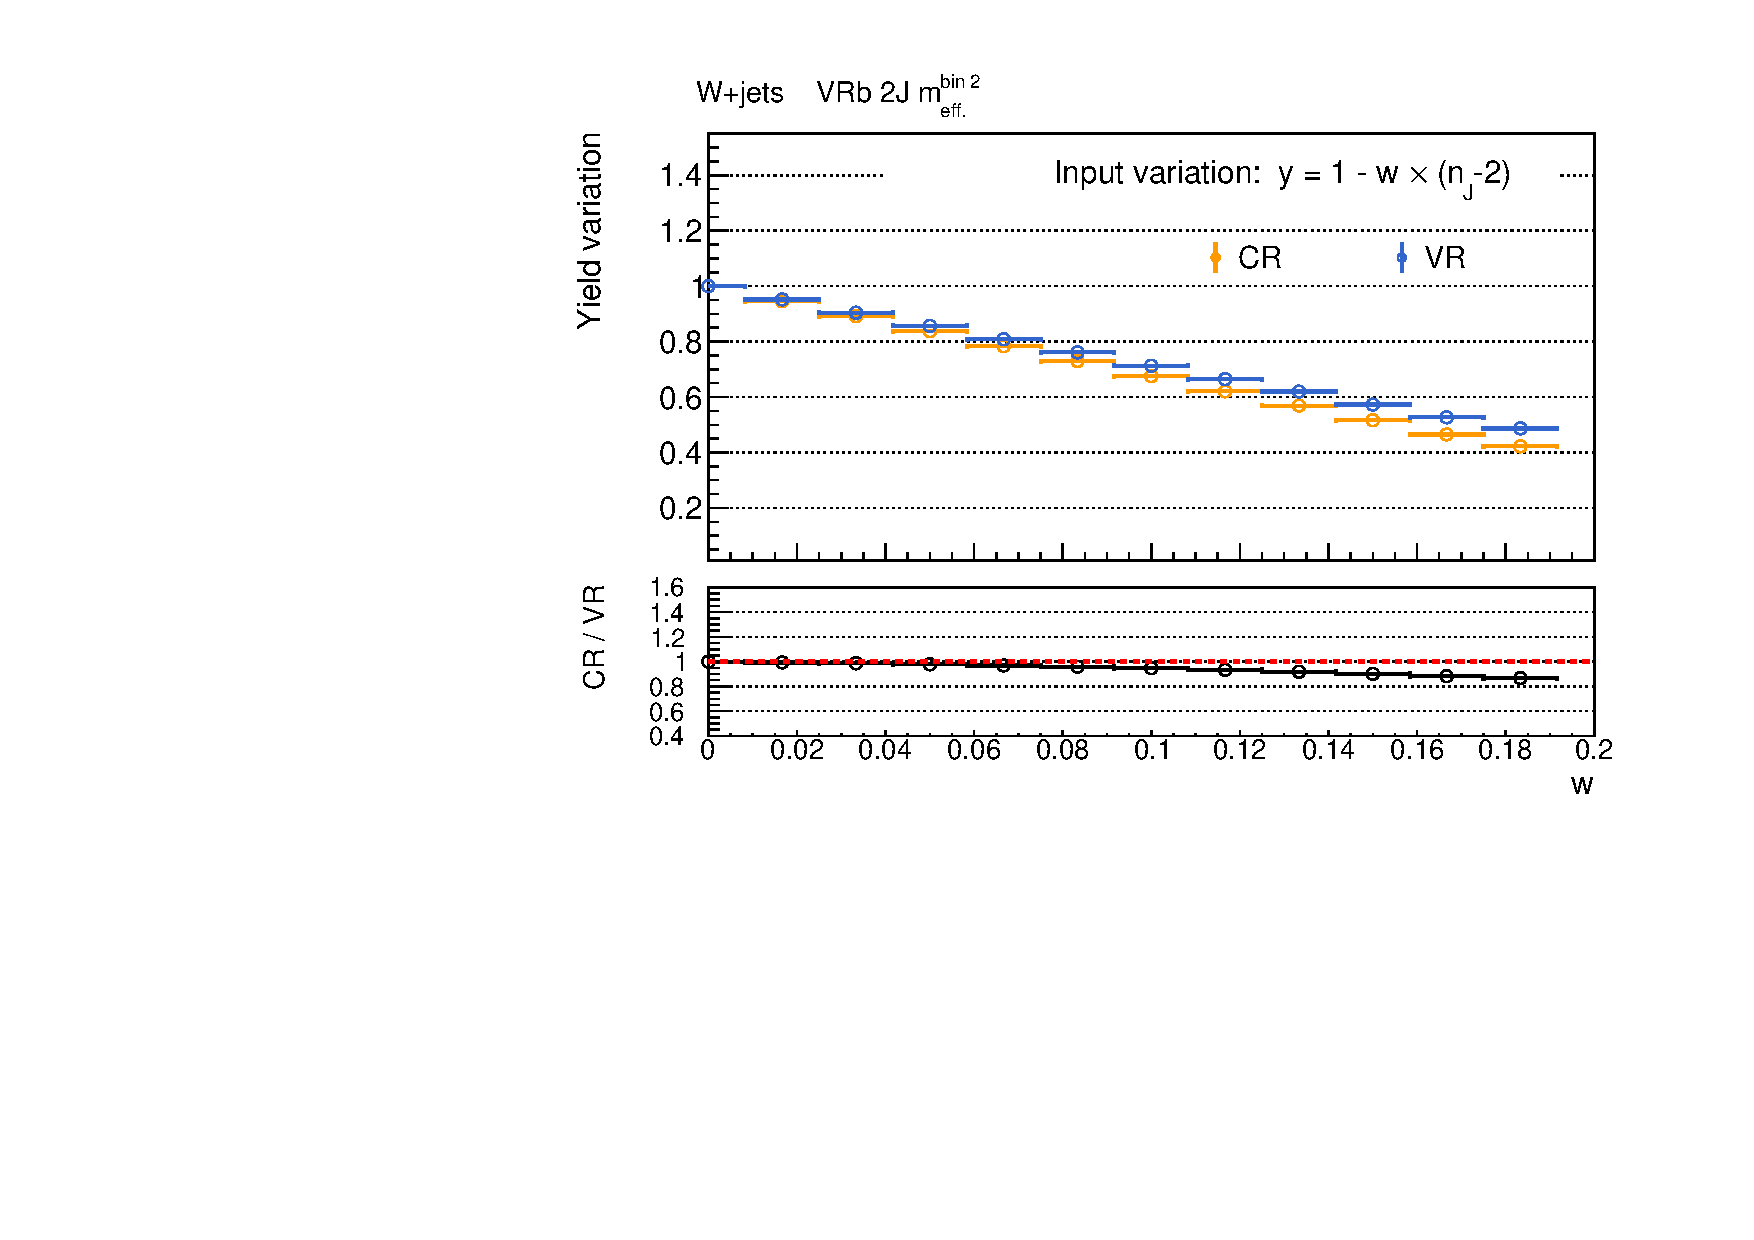
\includegraphics[width=0.488\textwidth]{figures/BGestimation/valid_extp/SFTF_wjets_VRb2JMEFF2_extp_var2J__nJet30.pdf}}
    \subfigure[]{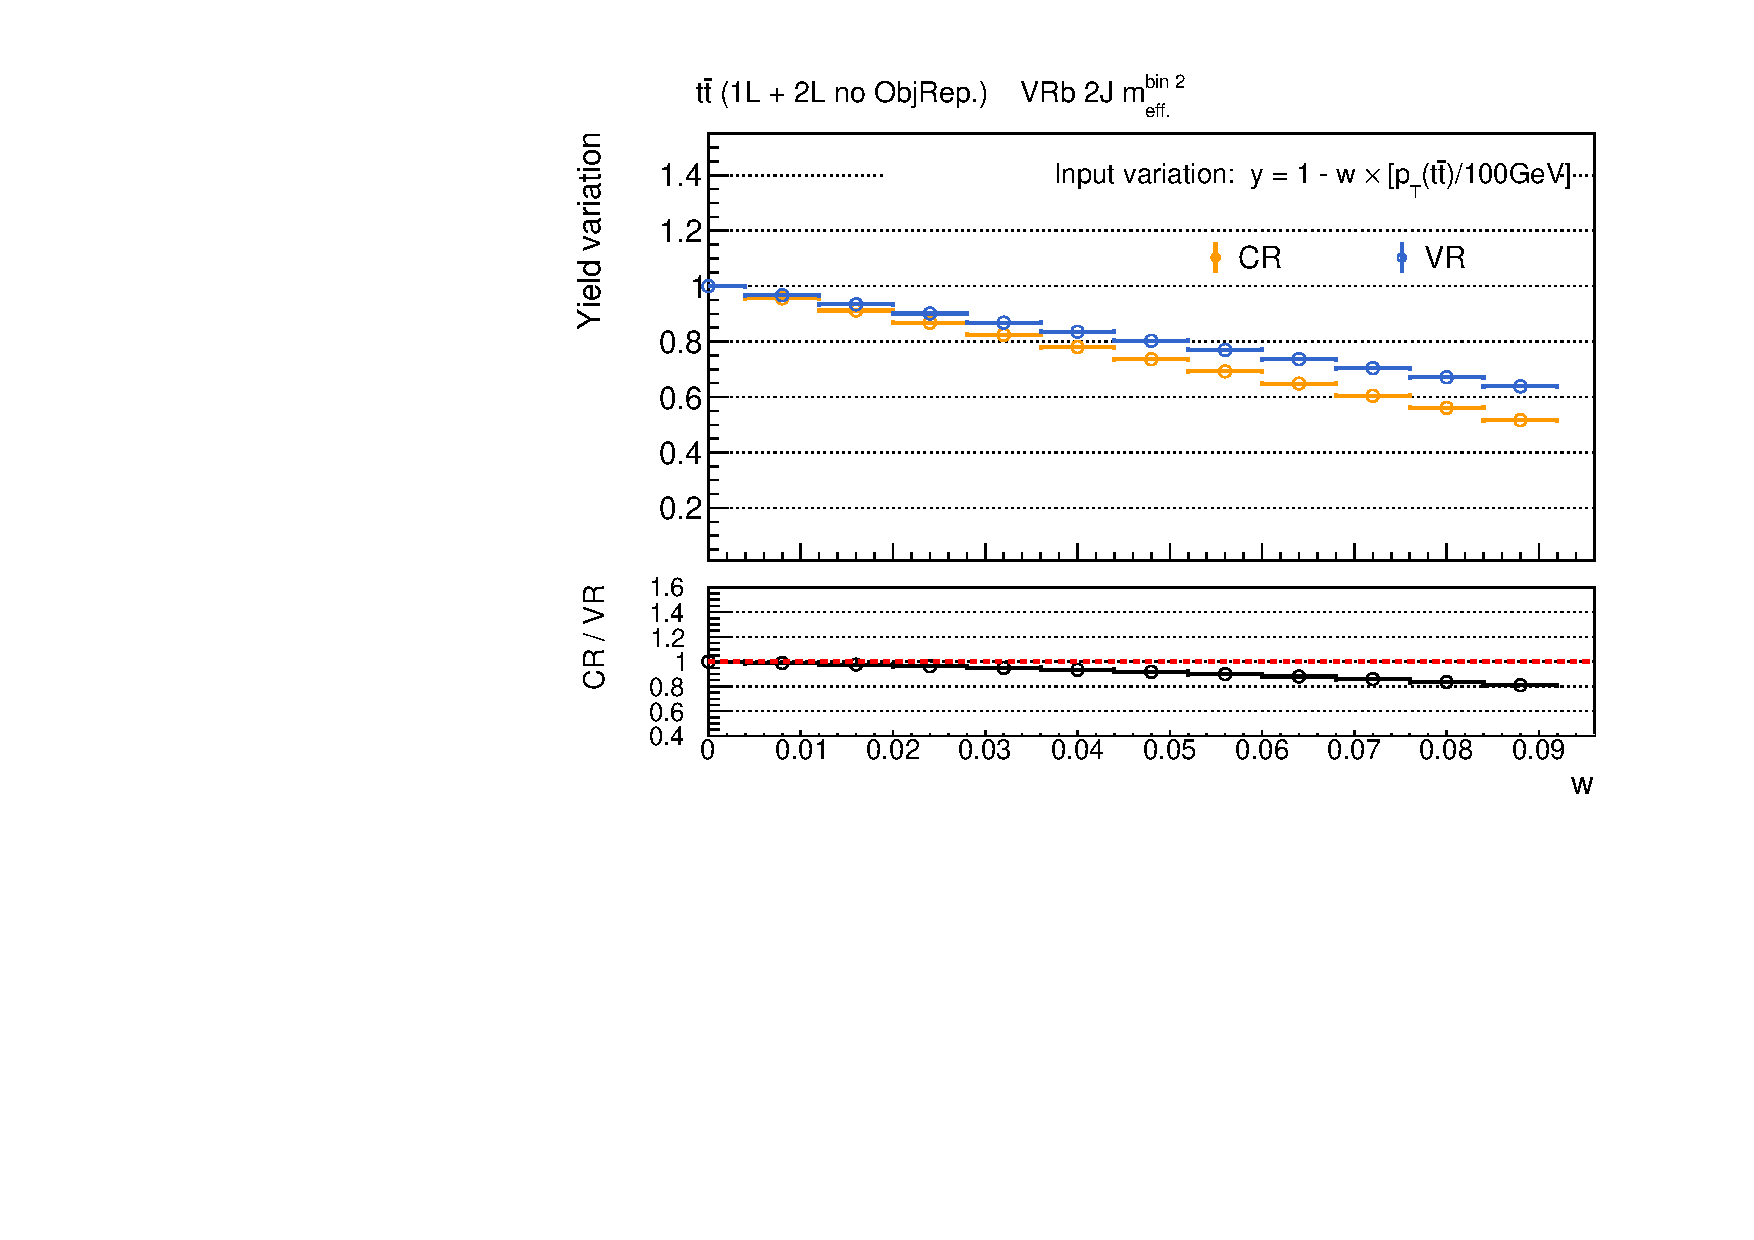
\includegraphics[width=0.488\textwidth]{figures/BGestimation/valid_extp/SFTF_ttNoObjRep_VRb2JMEFF2_extp_var2J__ttPt.pdf}}
    \subfigure[]{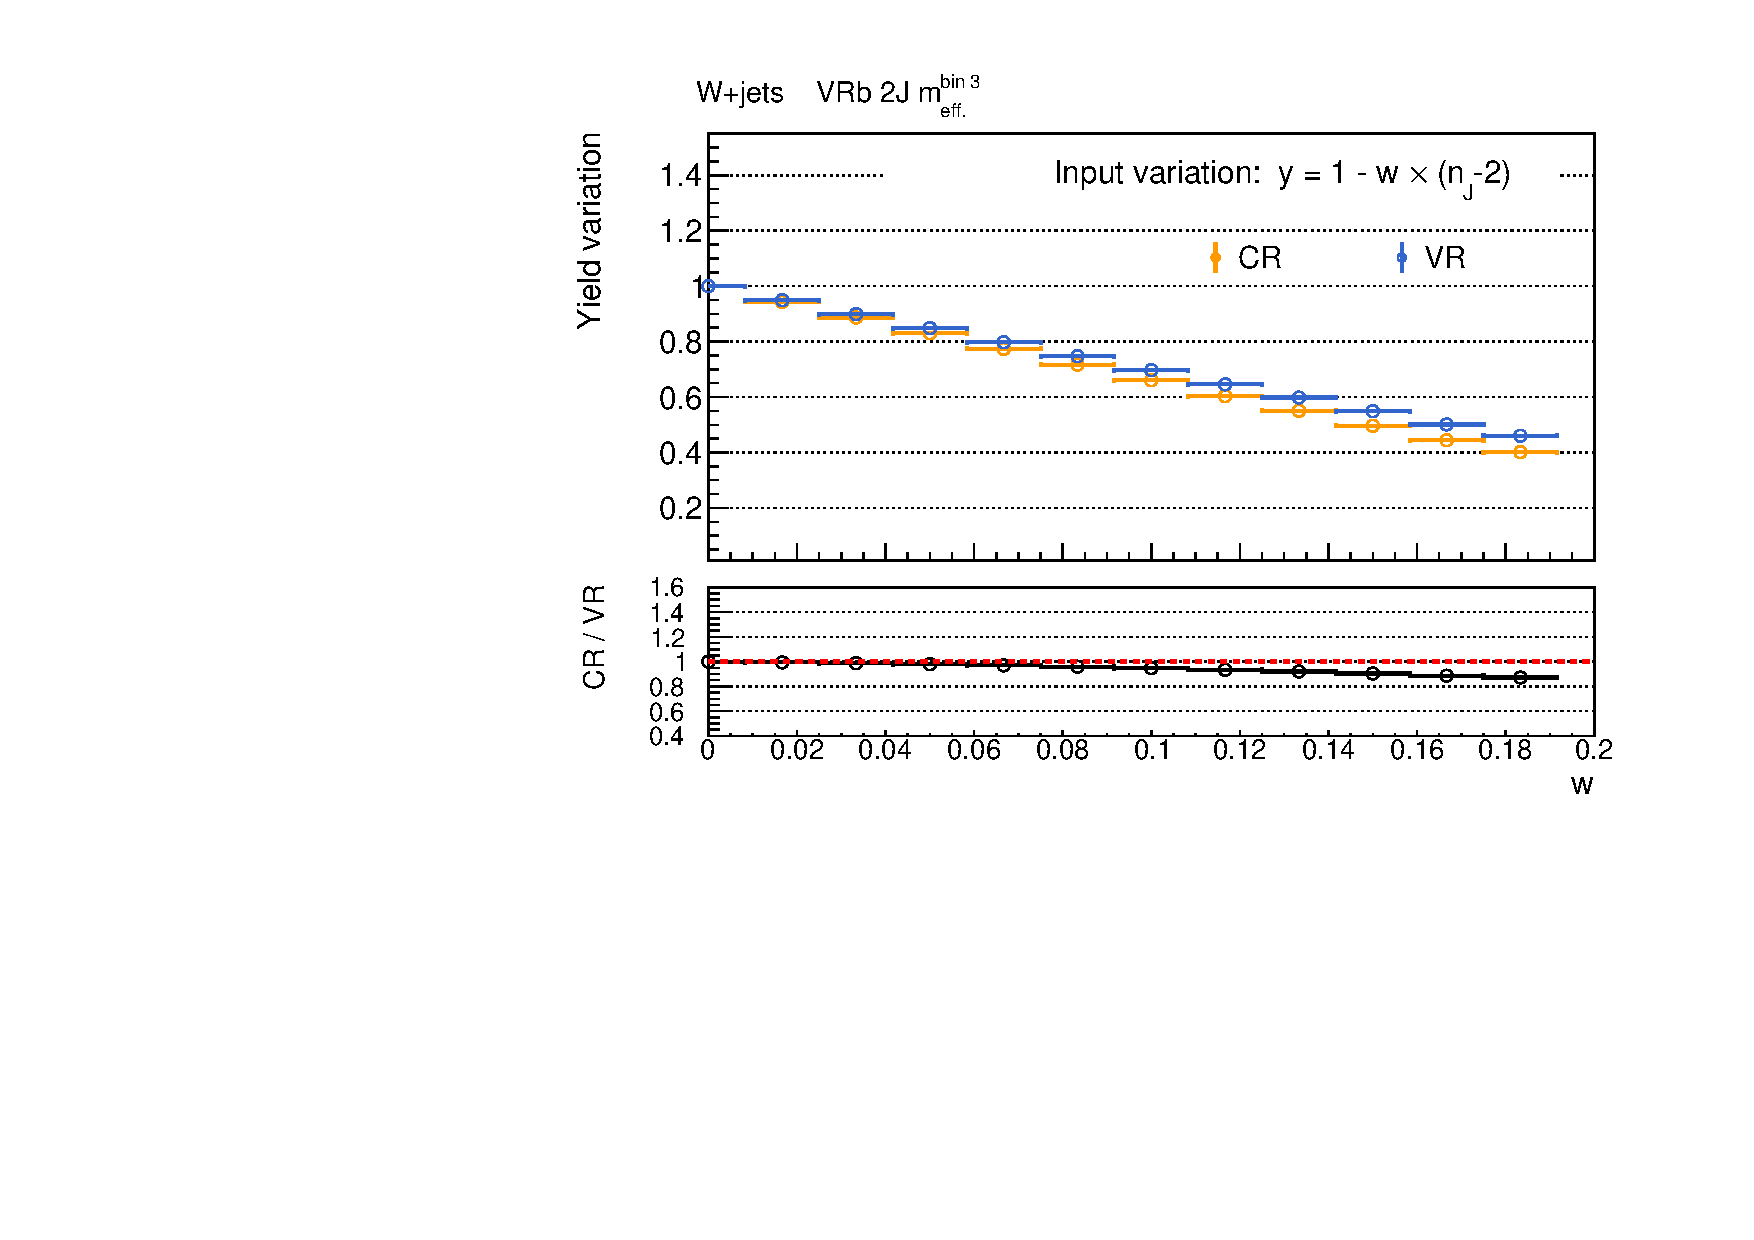
\includegraphics[width=0.488\textwidth]{figures/BGestimation/valid_extp/SFTF_wjets_VRb2JMEFF3_extp_var2J__nJet30.pdf}}
    \subfigure[]{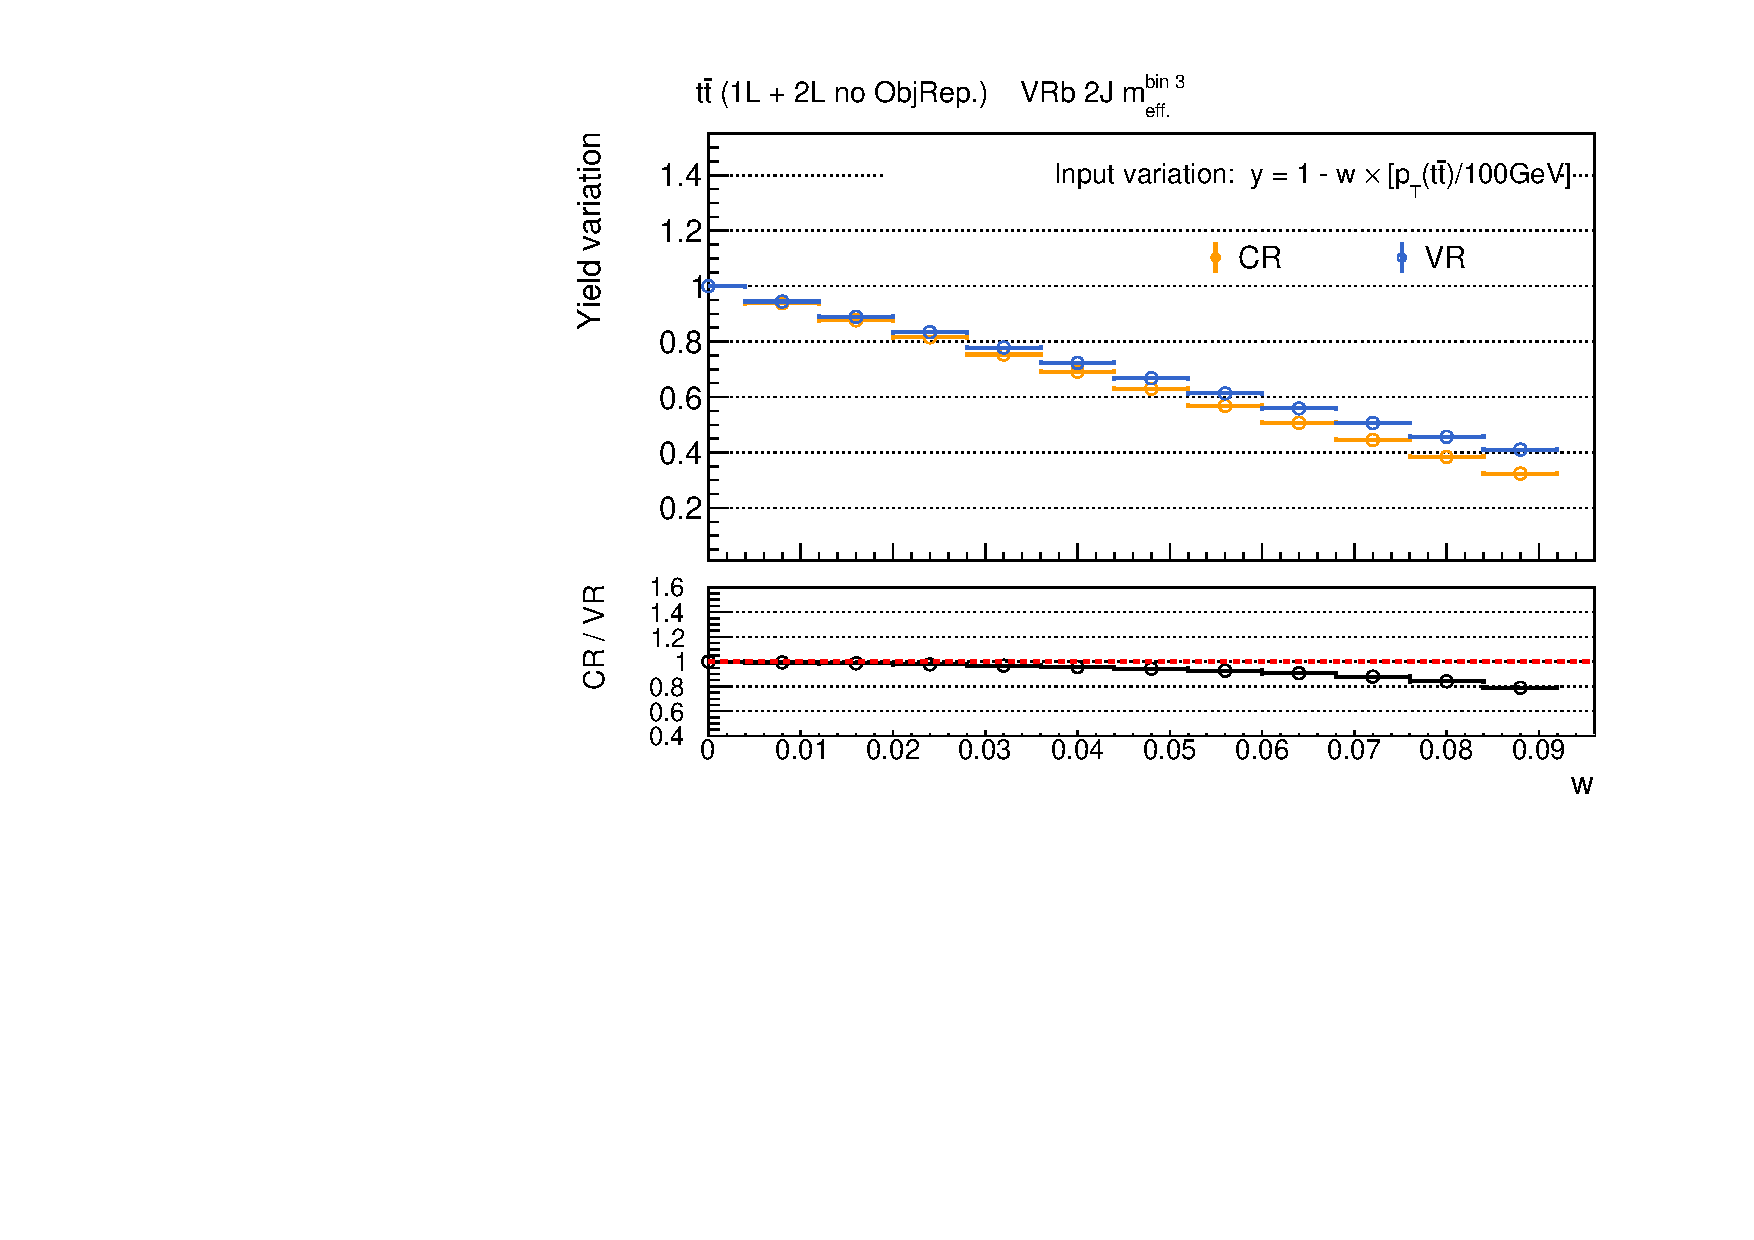
\includegraphics[width=0.488\textwidth]{figures/BGestimation/valid_extp/SFTF_ttNoObjRep_VRb2JMEFF3_extp_var2J__ttPt.pdf}}
 \caption{Extrapolation error in VRb/CR 2J. B-tagging requirement is removed. Top pannels show the yield variation of (a) $\wjets$ and (b) $\ttbar$ when injecting the variation by reweighting the MC with Eq. \ref{eq::BGestimation::injected_MCvariation}. Bottom rows are the relative difference in their response against the injected variation, namely the extrapolation errir. For the $\ttbar$ process, component estimated by the object replacement method is removed.  \label{fig::BGestimation::valid_extp_VRb2J} }
\end{figure}



%%%%%%%%%%%%%%%% VRb6J
\begin{figure}[h]
  \centering
    \subfigure[]{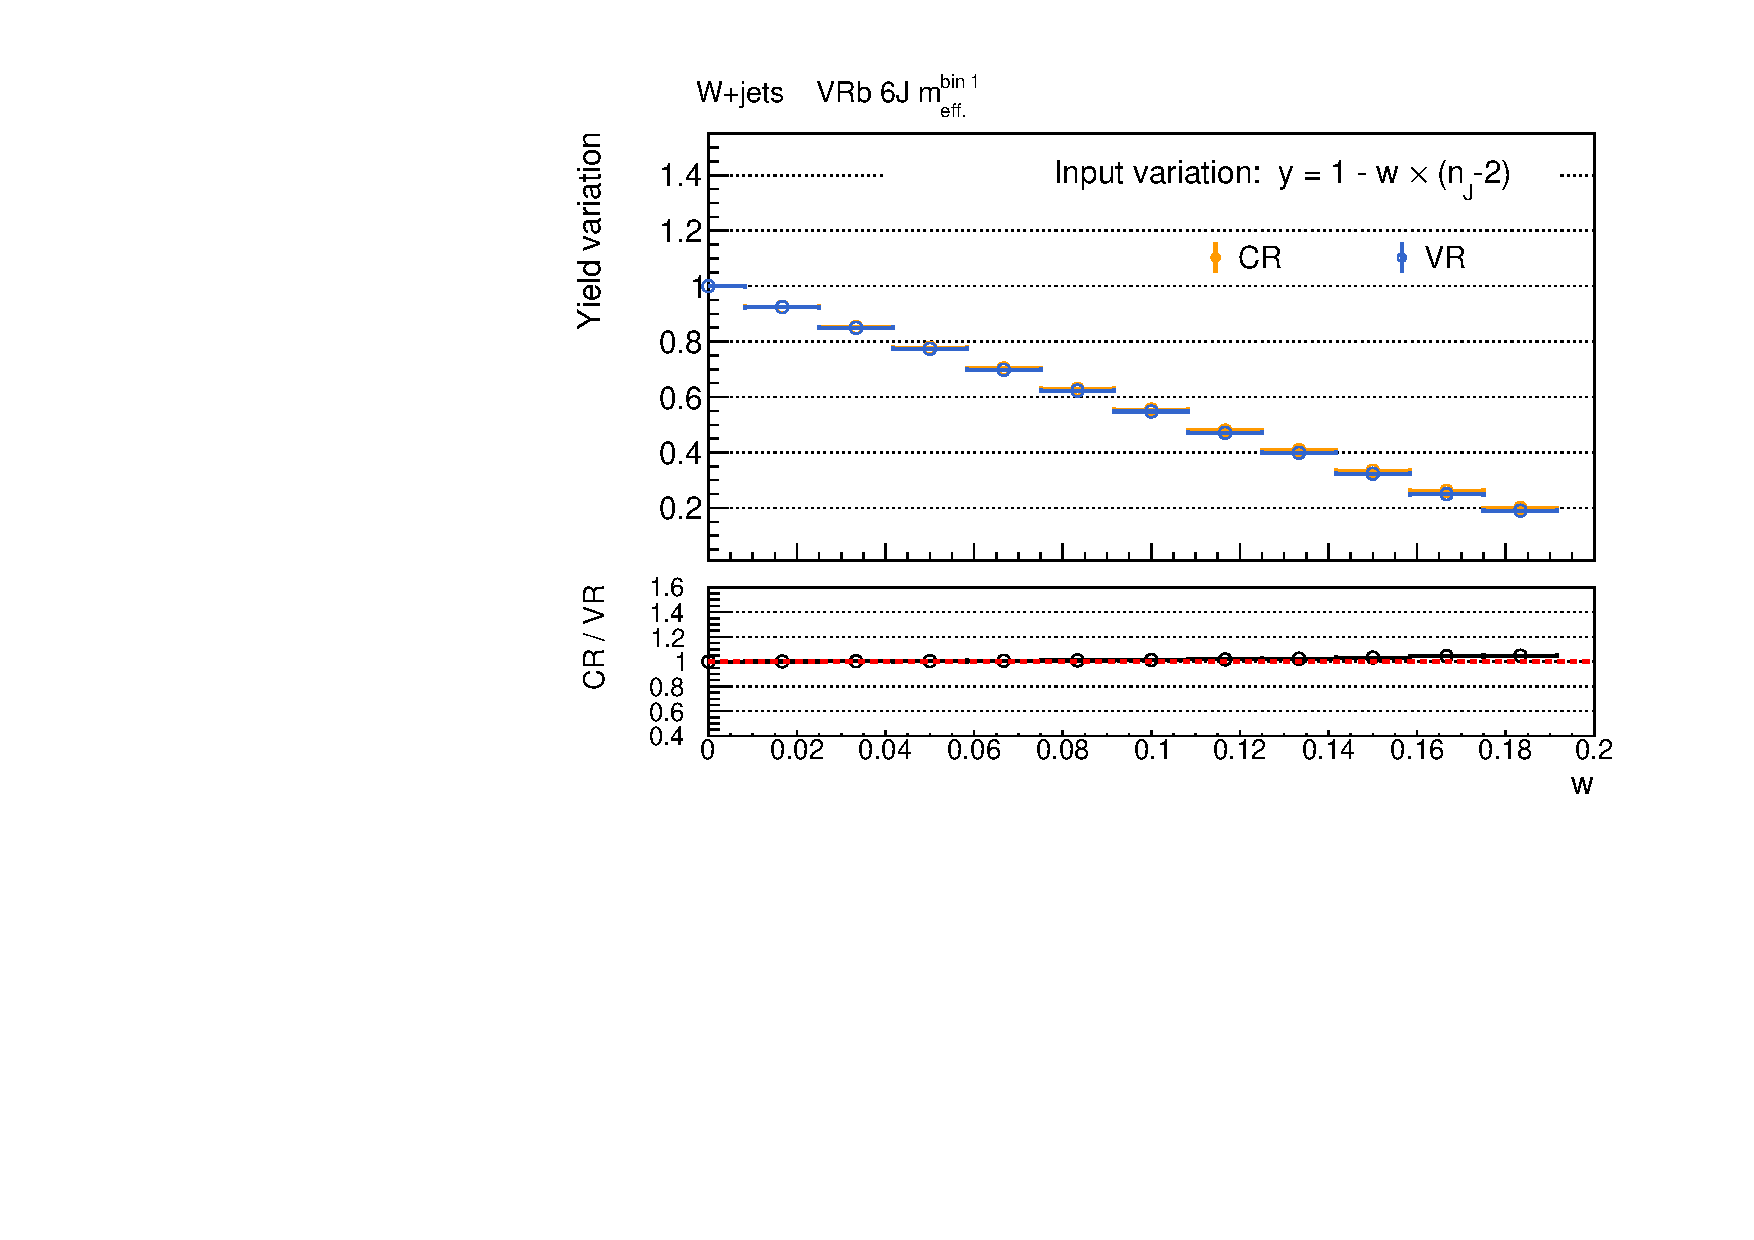
\includegraphics[width=0.488\textwidth]{figures/BGestimation/valid_extp/SFTF_wjets_VRb6JMEFF1_extp_var6J__nJet30.pdf}}
    \subfigure[]{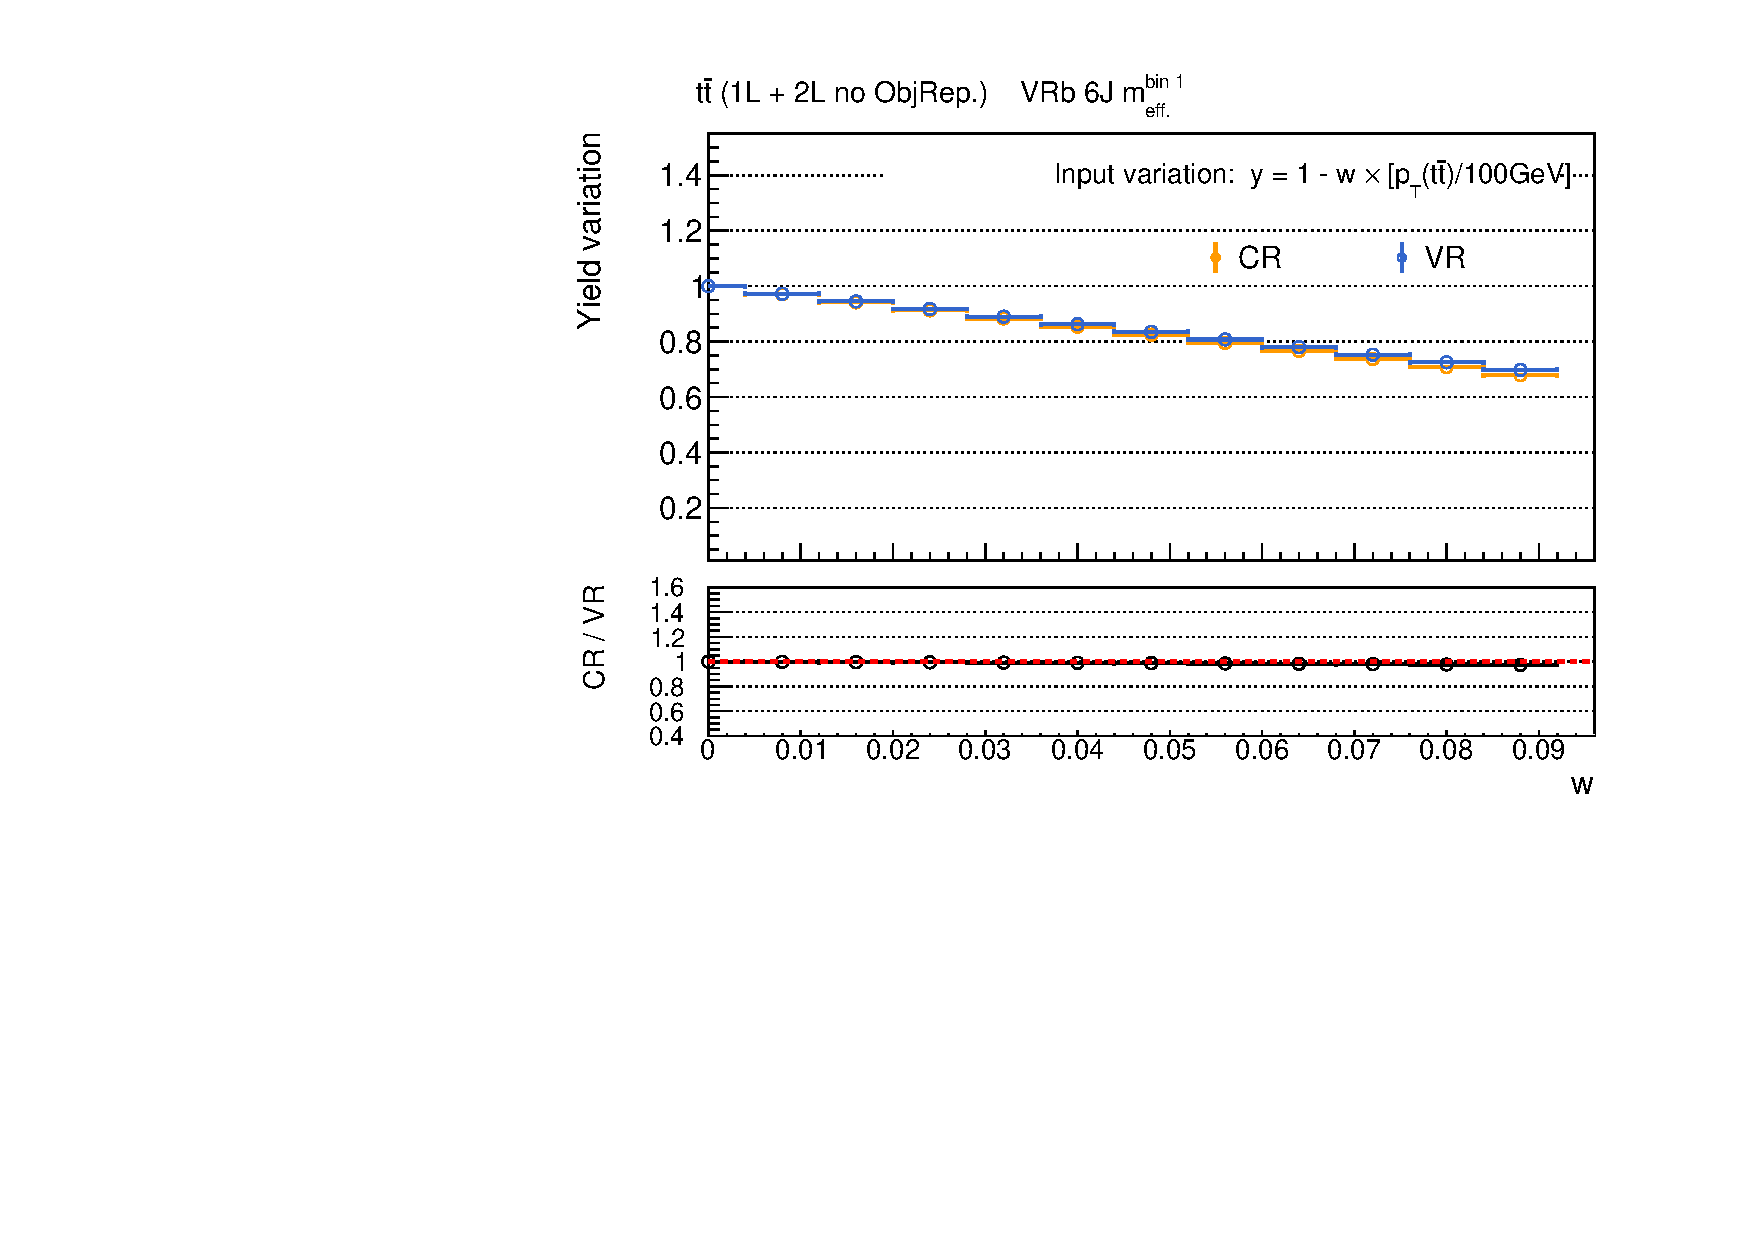
\includegraphics[width=0.488\textwidth]{figures/BGestimation/valid_extp/SFTF_ttNoObjRep_VRb6JMEFF1_extp_var6J__ttPt.pdf}}
    \subfigure[]{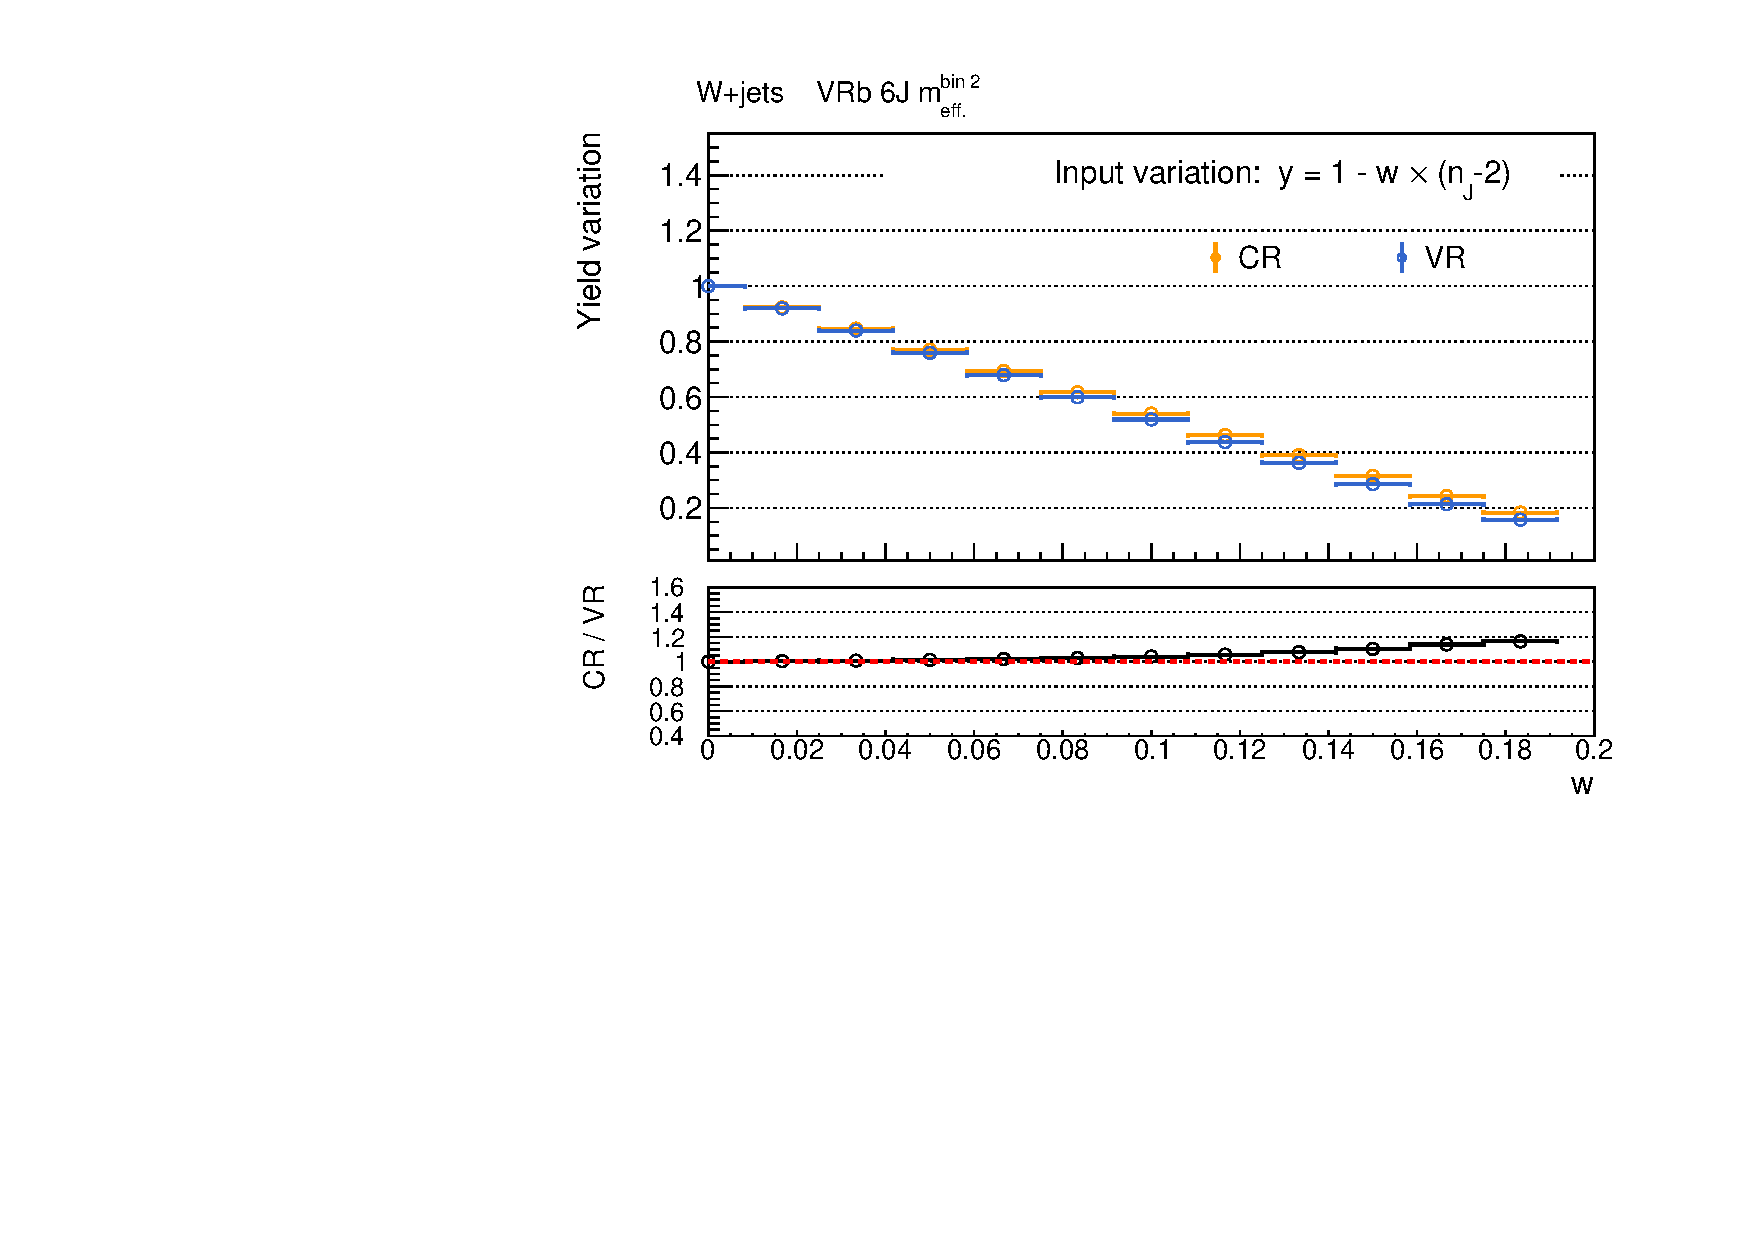
\includegraphics[width=0.488\textwidth]{figures/BGestimation/valid_extp/SFTF_wjets_VRb6JMEFF2_extp_var6J__nJet30.pdf}}
    \subfigure[]{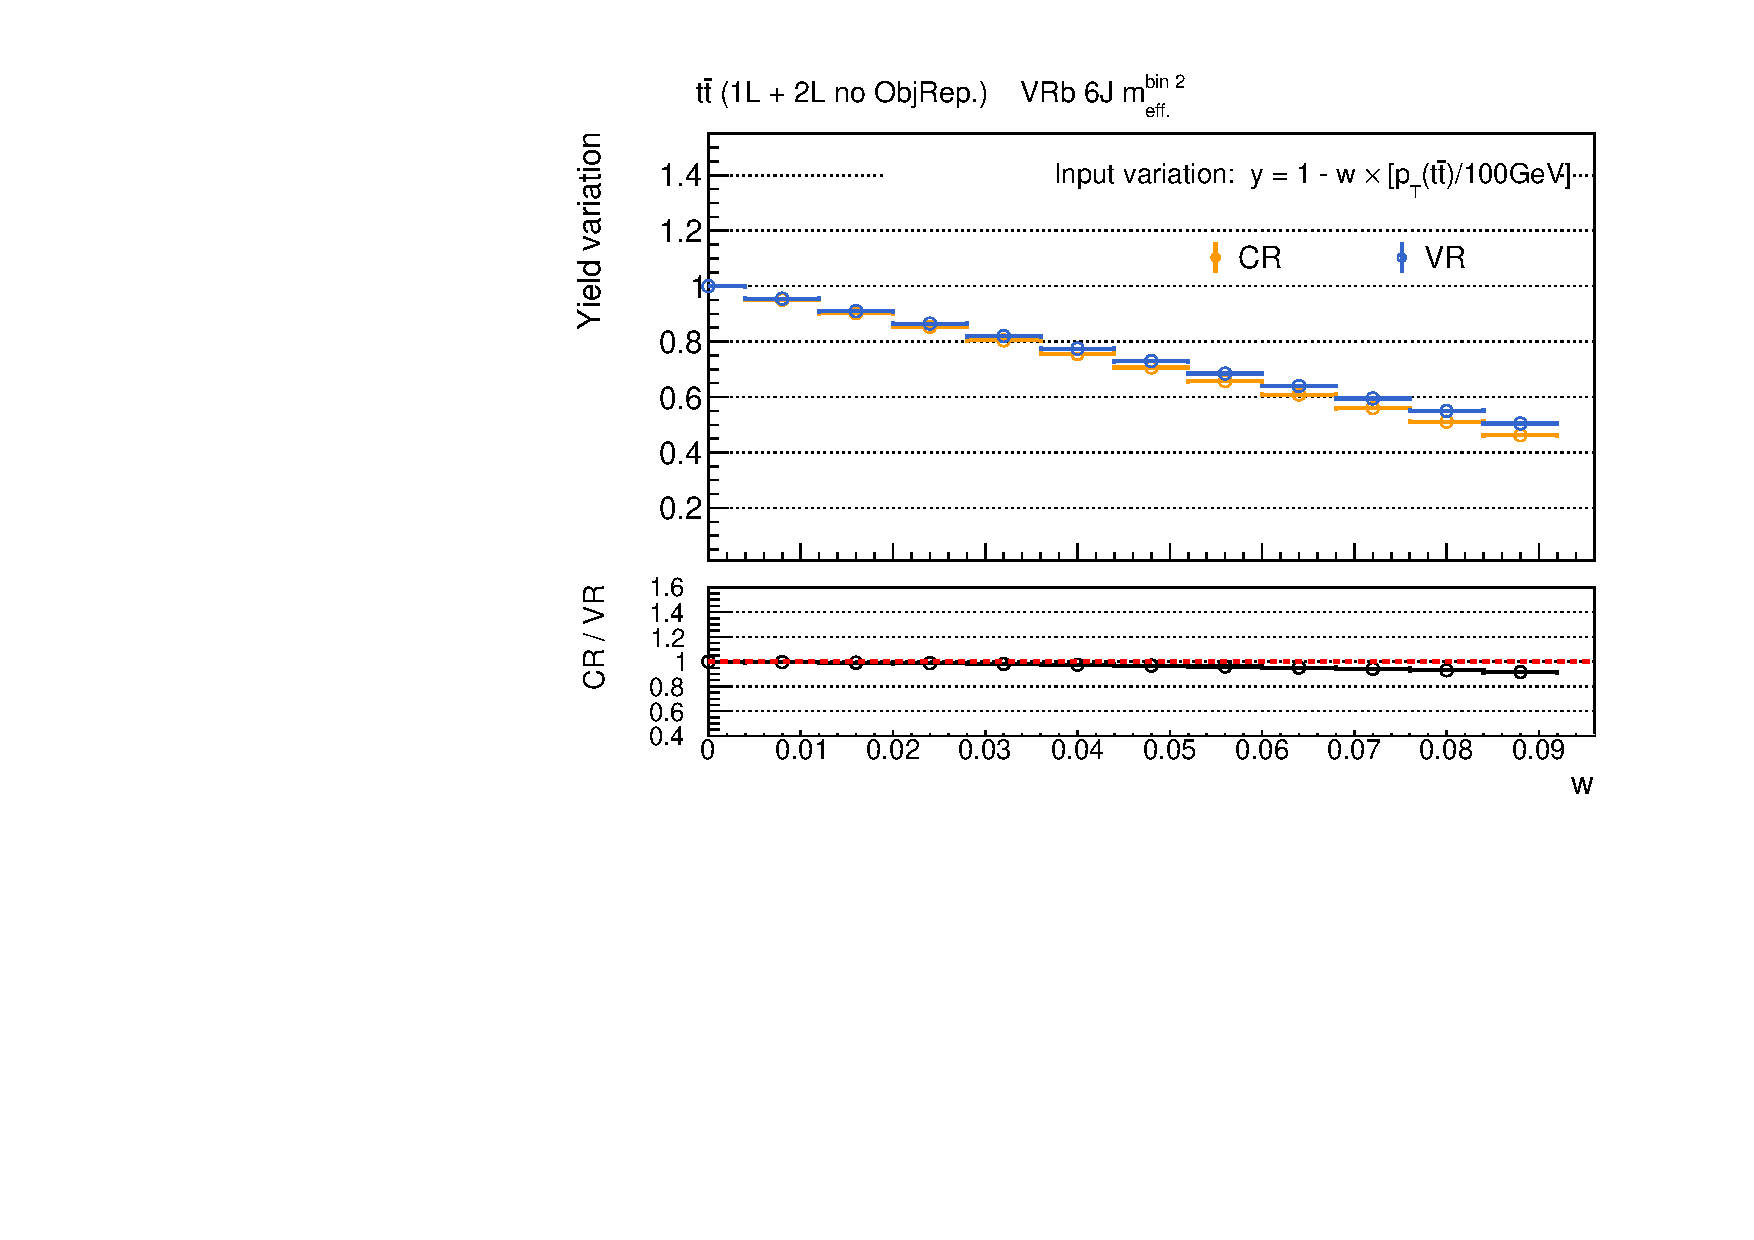
\includegraphics[width=0.488\textwidth]{figures/BGestimation/valid_extp/SFTF_ttNoObjRep_VRb6JMEFF2_extp_var6J__ttPt.pdf}}
    \subfigure[]{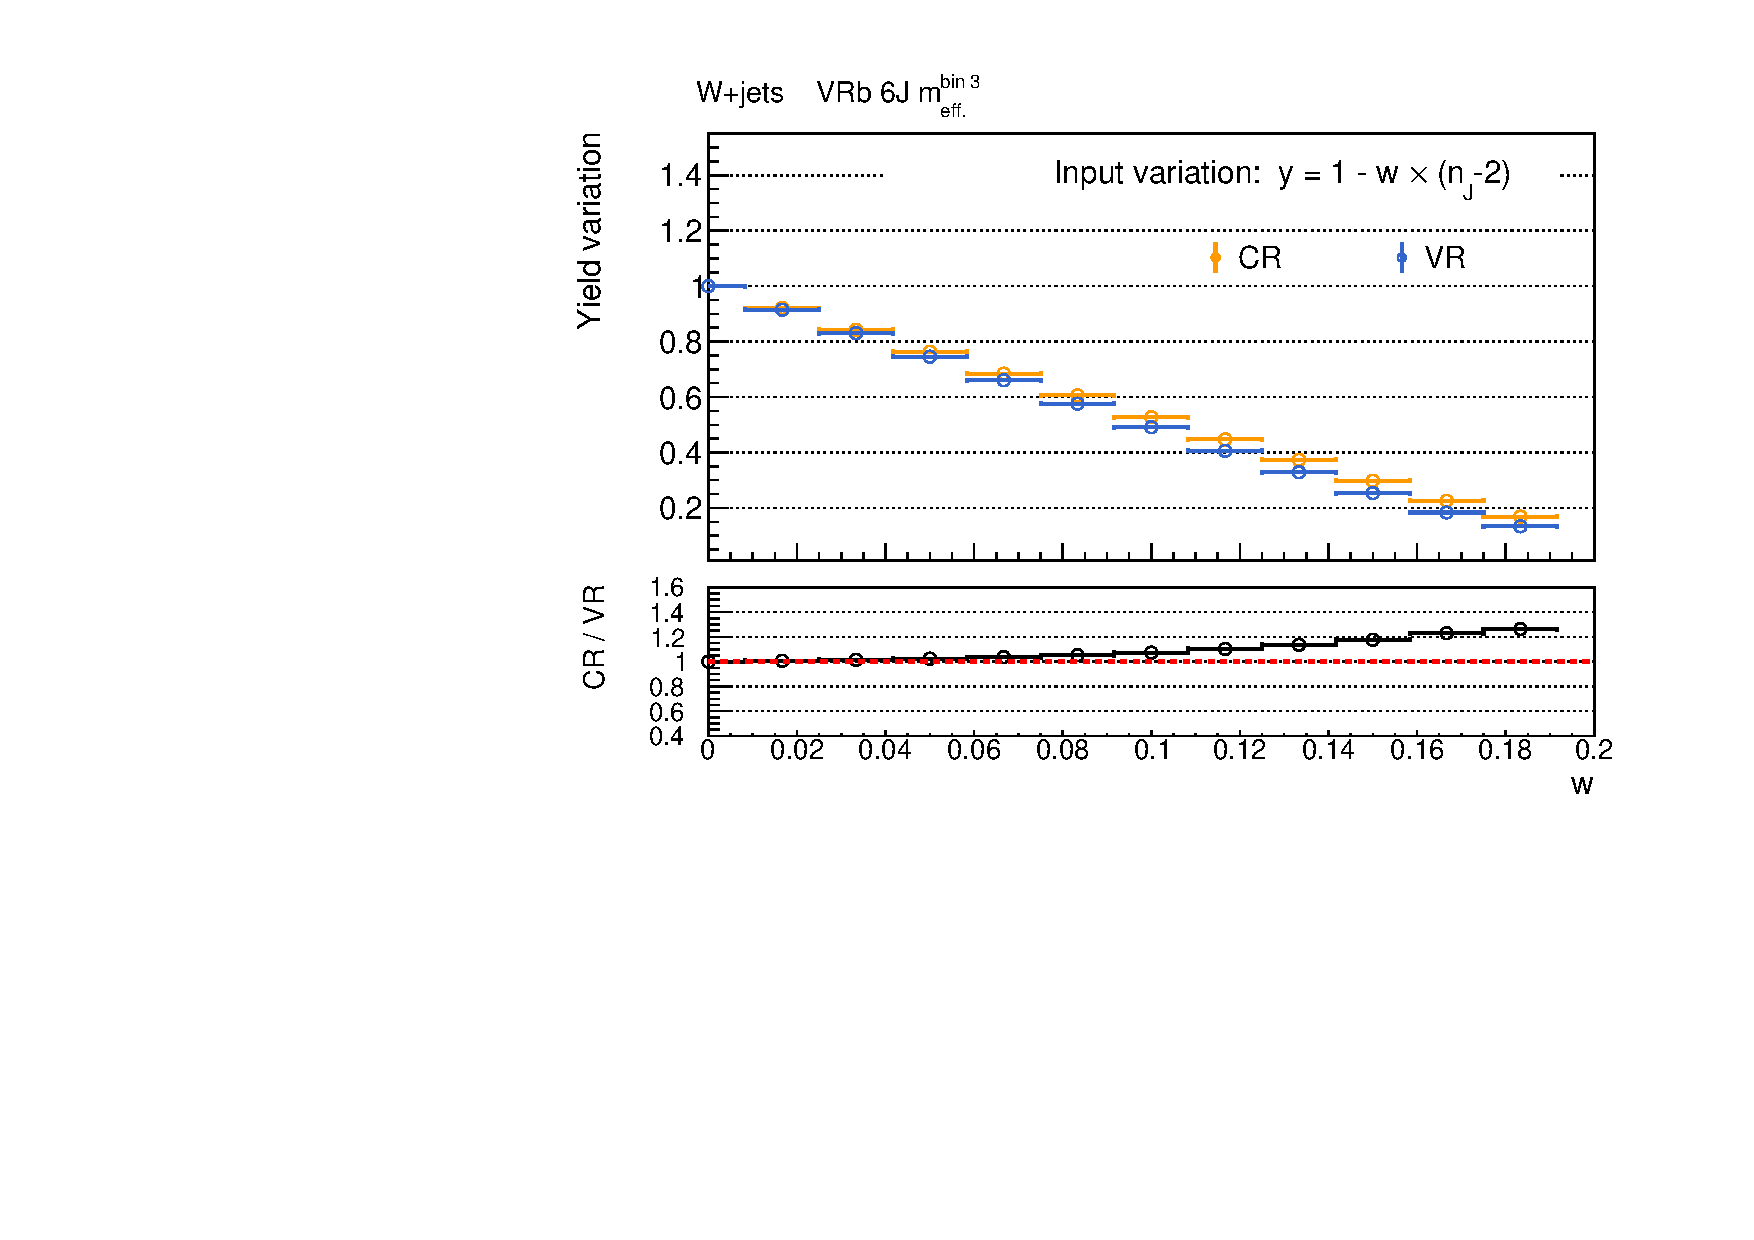
\includegraphics[width=0.488\textwidth]{figures/BGestimation/valid_extp/SFTF_wjets_VRb6JMEFF3_extp_var6J__nJet30.pdf}}
    \subfigure[]{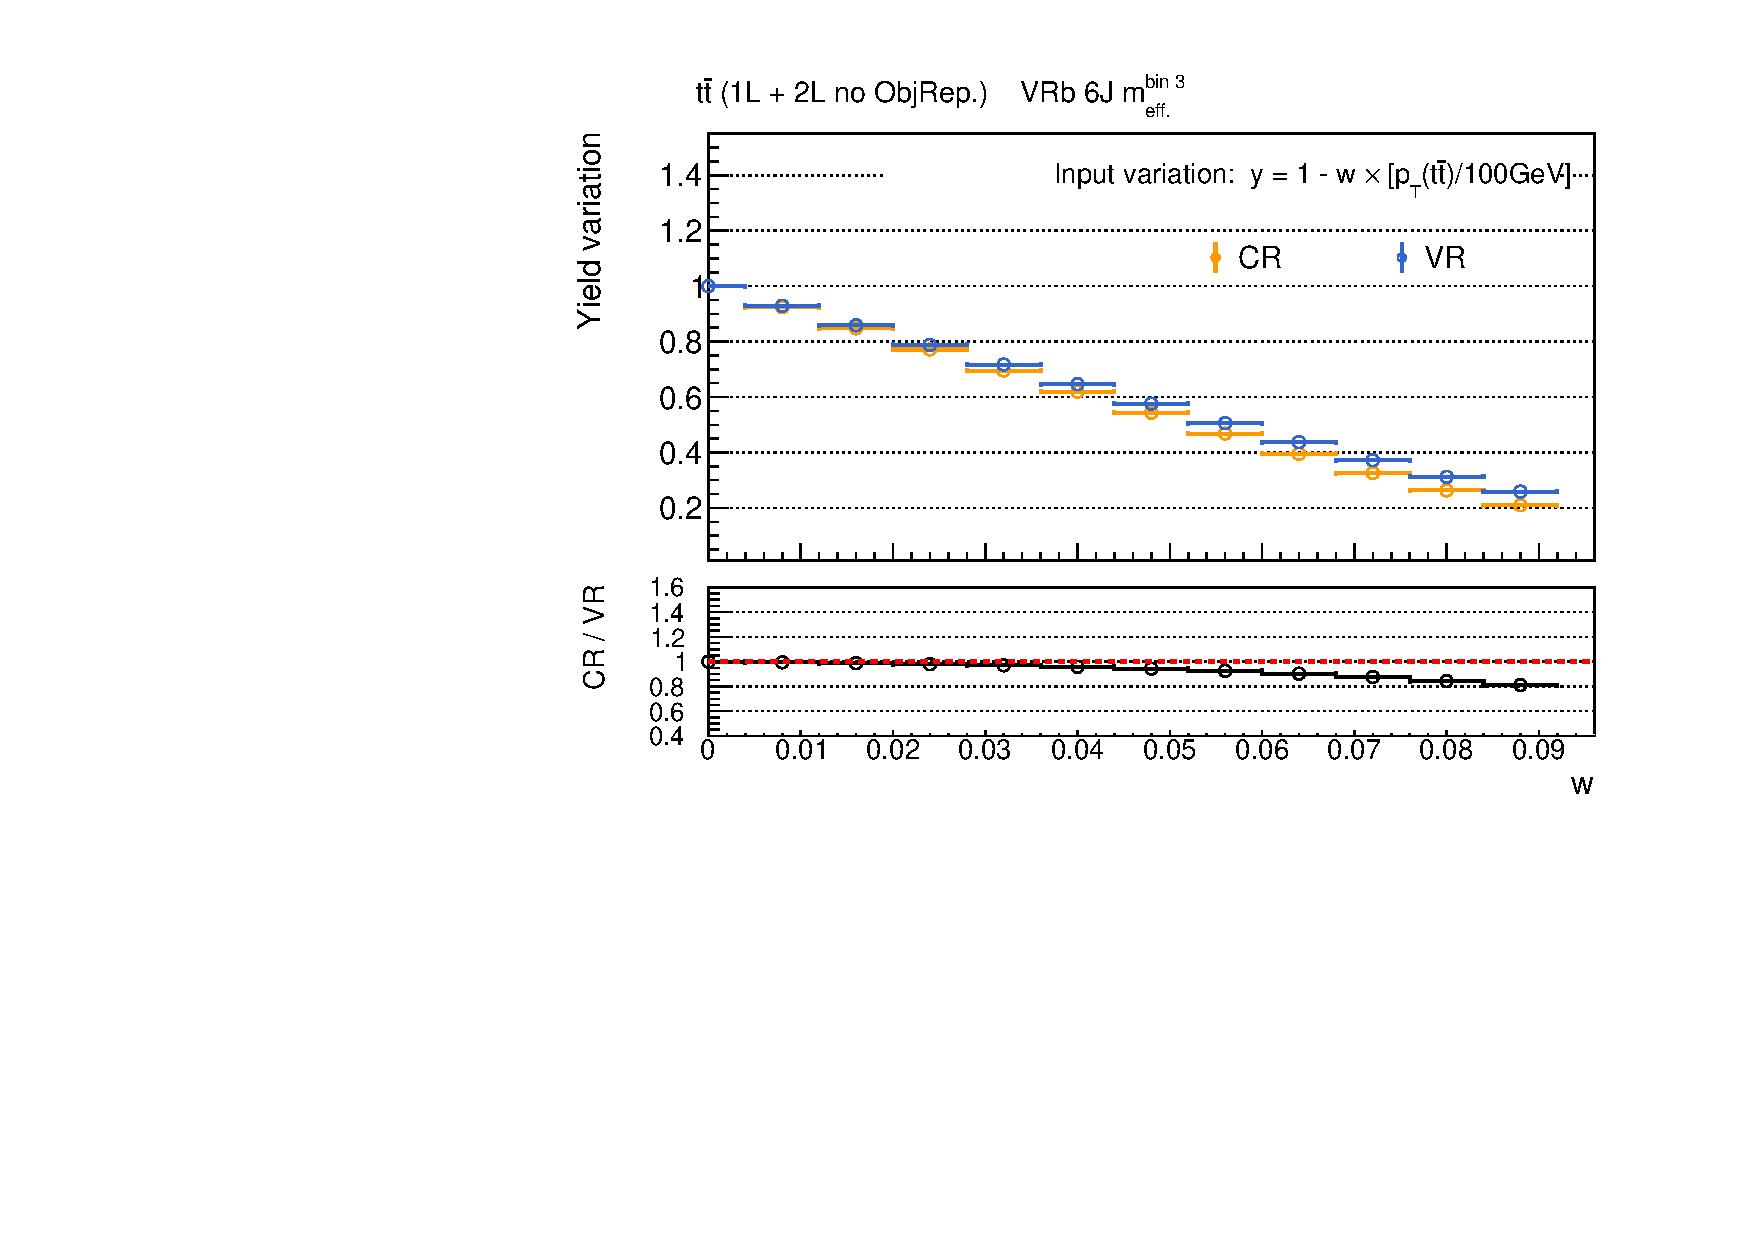
\includegraphics[width=0.488\textwidth]{figures/BGestimation/valid_extp/SFTF_ttNoObjRep_VRb6JMEFF3_extp_var6J__ttPt.pdf}}
 \caption{Extrapolation error in VRb/CR 6J. B-tagging requirement is removed. Top pannels show the yield variation of (a) $\wjets$ and (b) $\ttbar$ when injecting the variation by reweighting the MC with Eq. \ref{eq::BGestimation::injected_MCvariation}. Bottom rows are the relative difference in their response against the injected variation, namely the extrapolation errir. For the $\ttbar$ process, component estimated by the object replacement method is removed.  \label{fig::BGestimation::valid_extp_VRb6J} }
\end{figure}


%%%%%%%%%%%%%%%% Lowx
\begin{figure}[h]
  \centering
    \subfigure[]{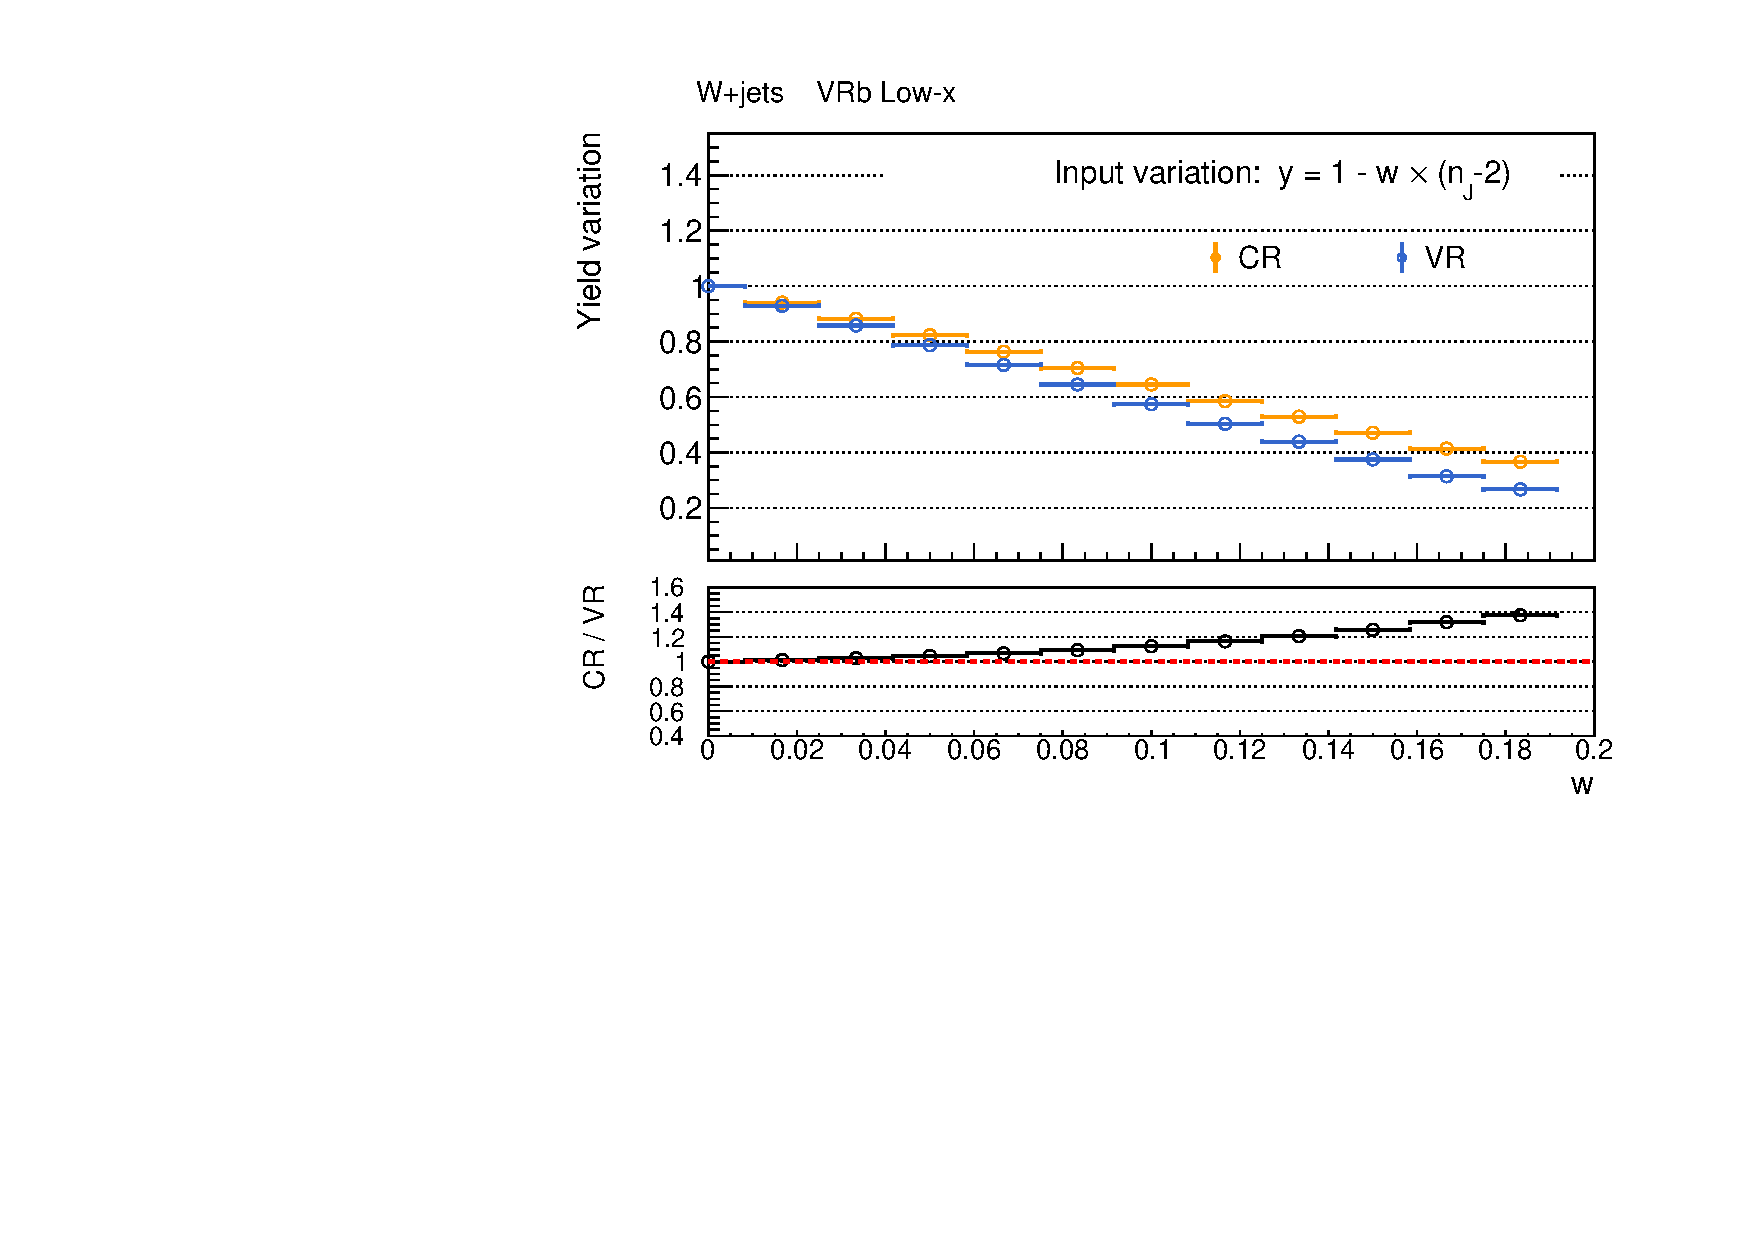
\includegraphics[width=0.488\textwidth]{figures/BGestimation/valid_extp/SFTF_wjets_VRbLowx_extp_varLowx__nJet30.pdf}}
    \subfigure[]{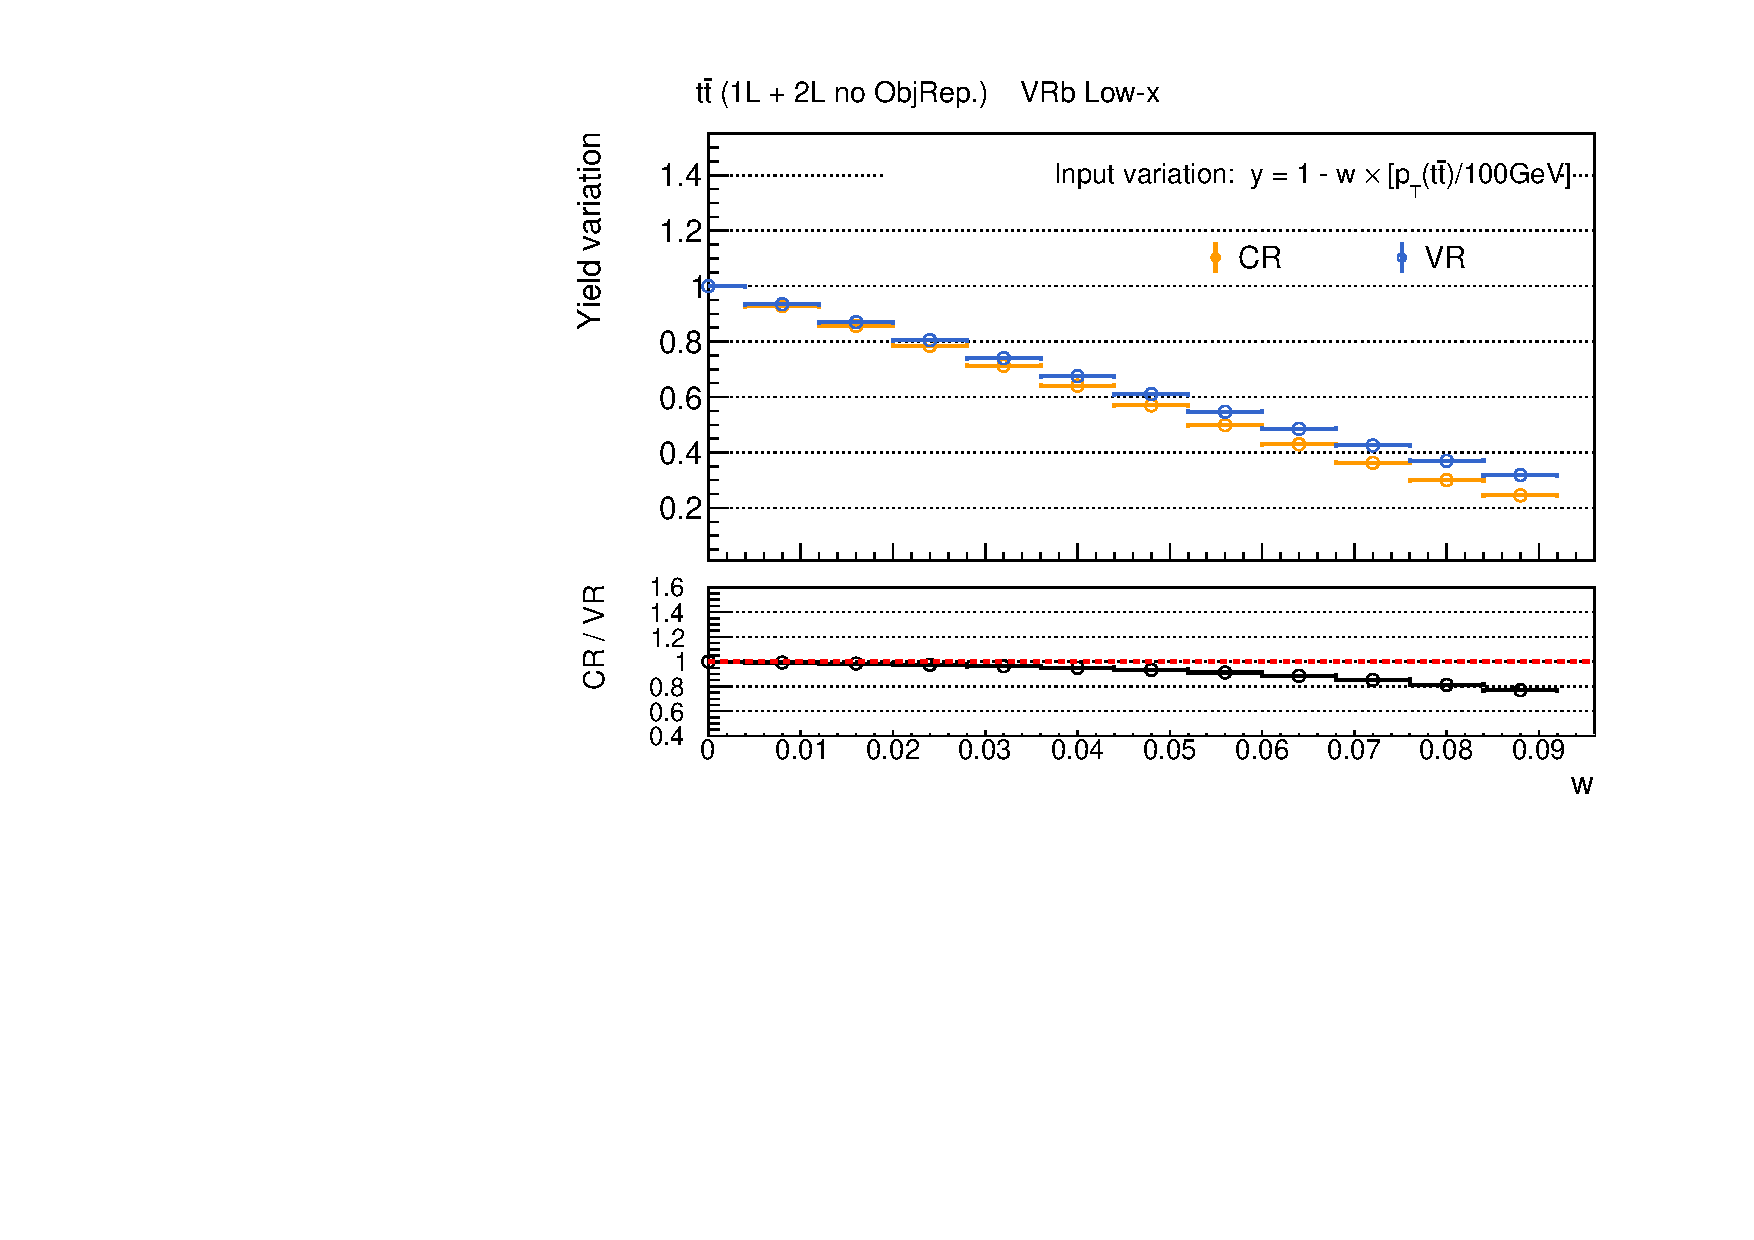
\includegraphics[width=0.488\textwidth]{figures/BGestimation/valid_extp/SFTF_ttNoObjRep_VRbLowx_extp_varLowx__ttPt.pdf}}

%%%%%%%%%%%%%%%% Highx
    \subfigure[]{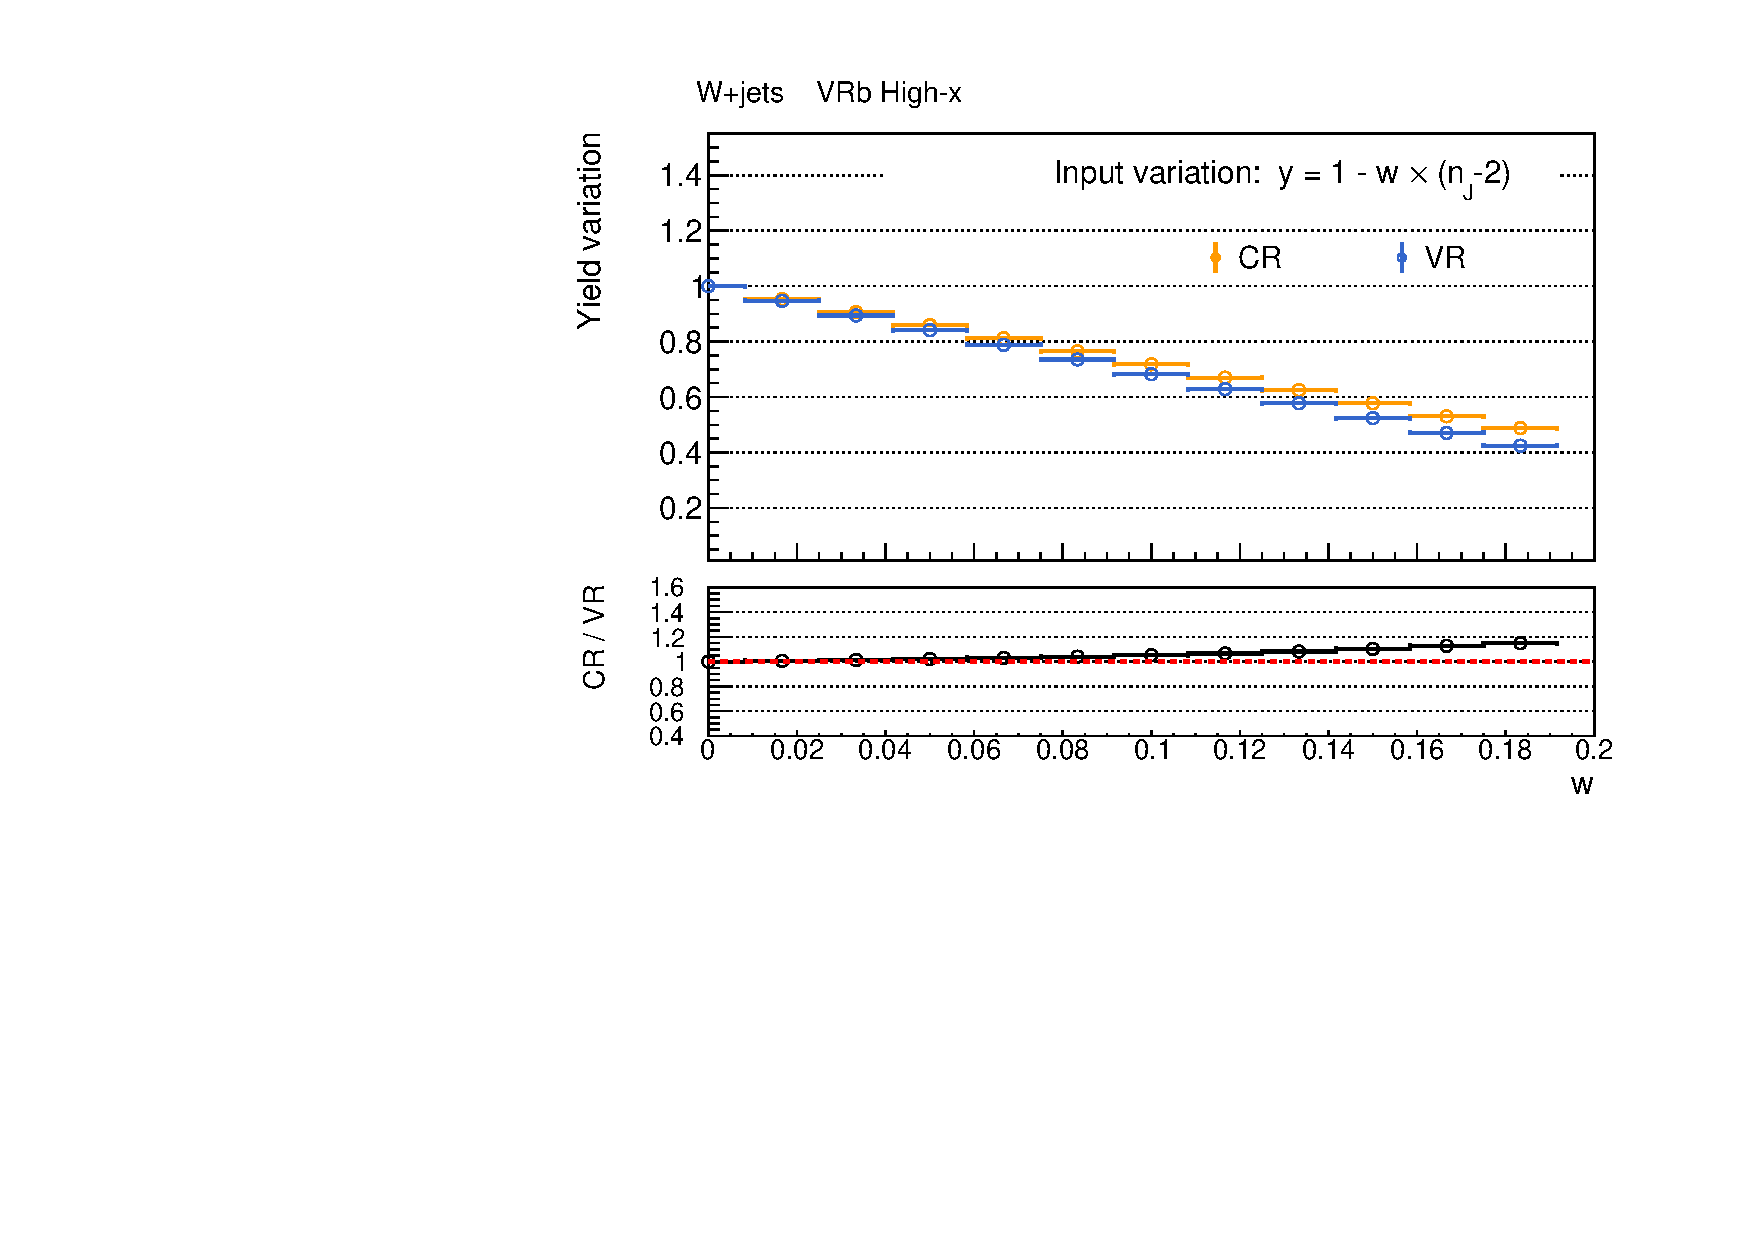
\includegraphics[width=0.488\textwidth]{figures/BGestimation/valid_extp/SFTF_wjets_VRbHighx_extp_varHighx__nJet30.pdf}}
    \subfigure[]{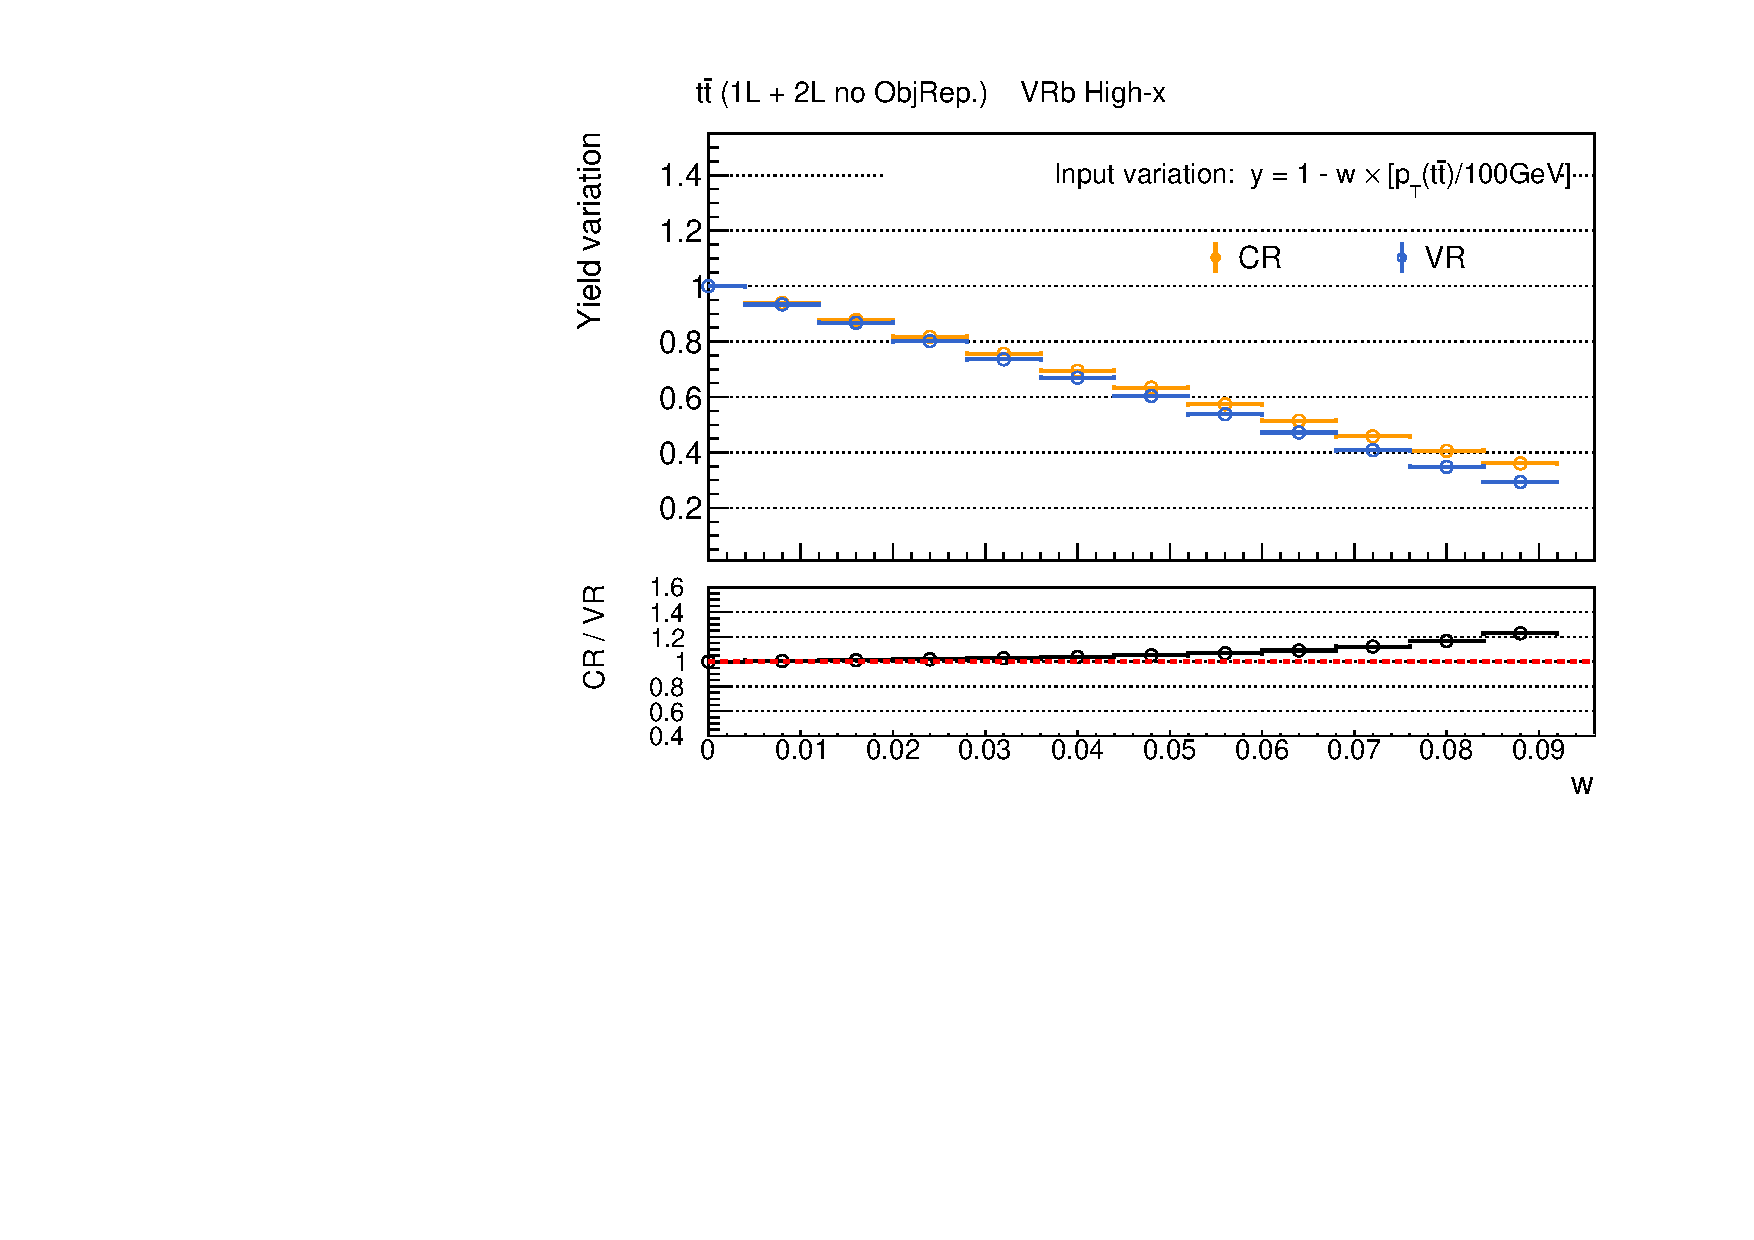
\includegraphics[width=0.488\textwidth]{figures/BGestimation/valid_extp/SFTF_ttNoObjRep_VRbHighx_extp_varHighx__ttPt.pdf}}
 \caption{Extrapolation error in VRb/CR (a)(b) Low-x, and (c)(d) High-x. B-tagging requirement is removed. Top pannels show the yield variation of $\wjets$ (left) and $\ttbar$ (right) when injecting the variation by reweighting the MC with Eq. \ref{eq::BGestimation::injected_MCvariation}. Bottom rows are the relative difference in their response against the injected variation, namely the extrapolation errir. For the $\ttbar$ process, component estimated by the object replacement method is removed.  \label{fig::BGestimation::valid_extp_VRb6J} }
\end{figure}


%%%%%%%%%%%%%%%% 3B
\begin{figure}[h]
  \centering
    \subfigure[]{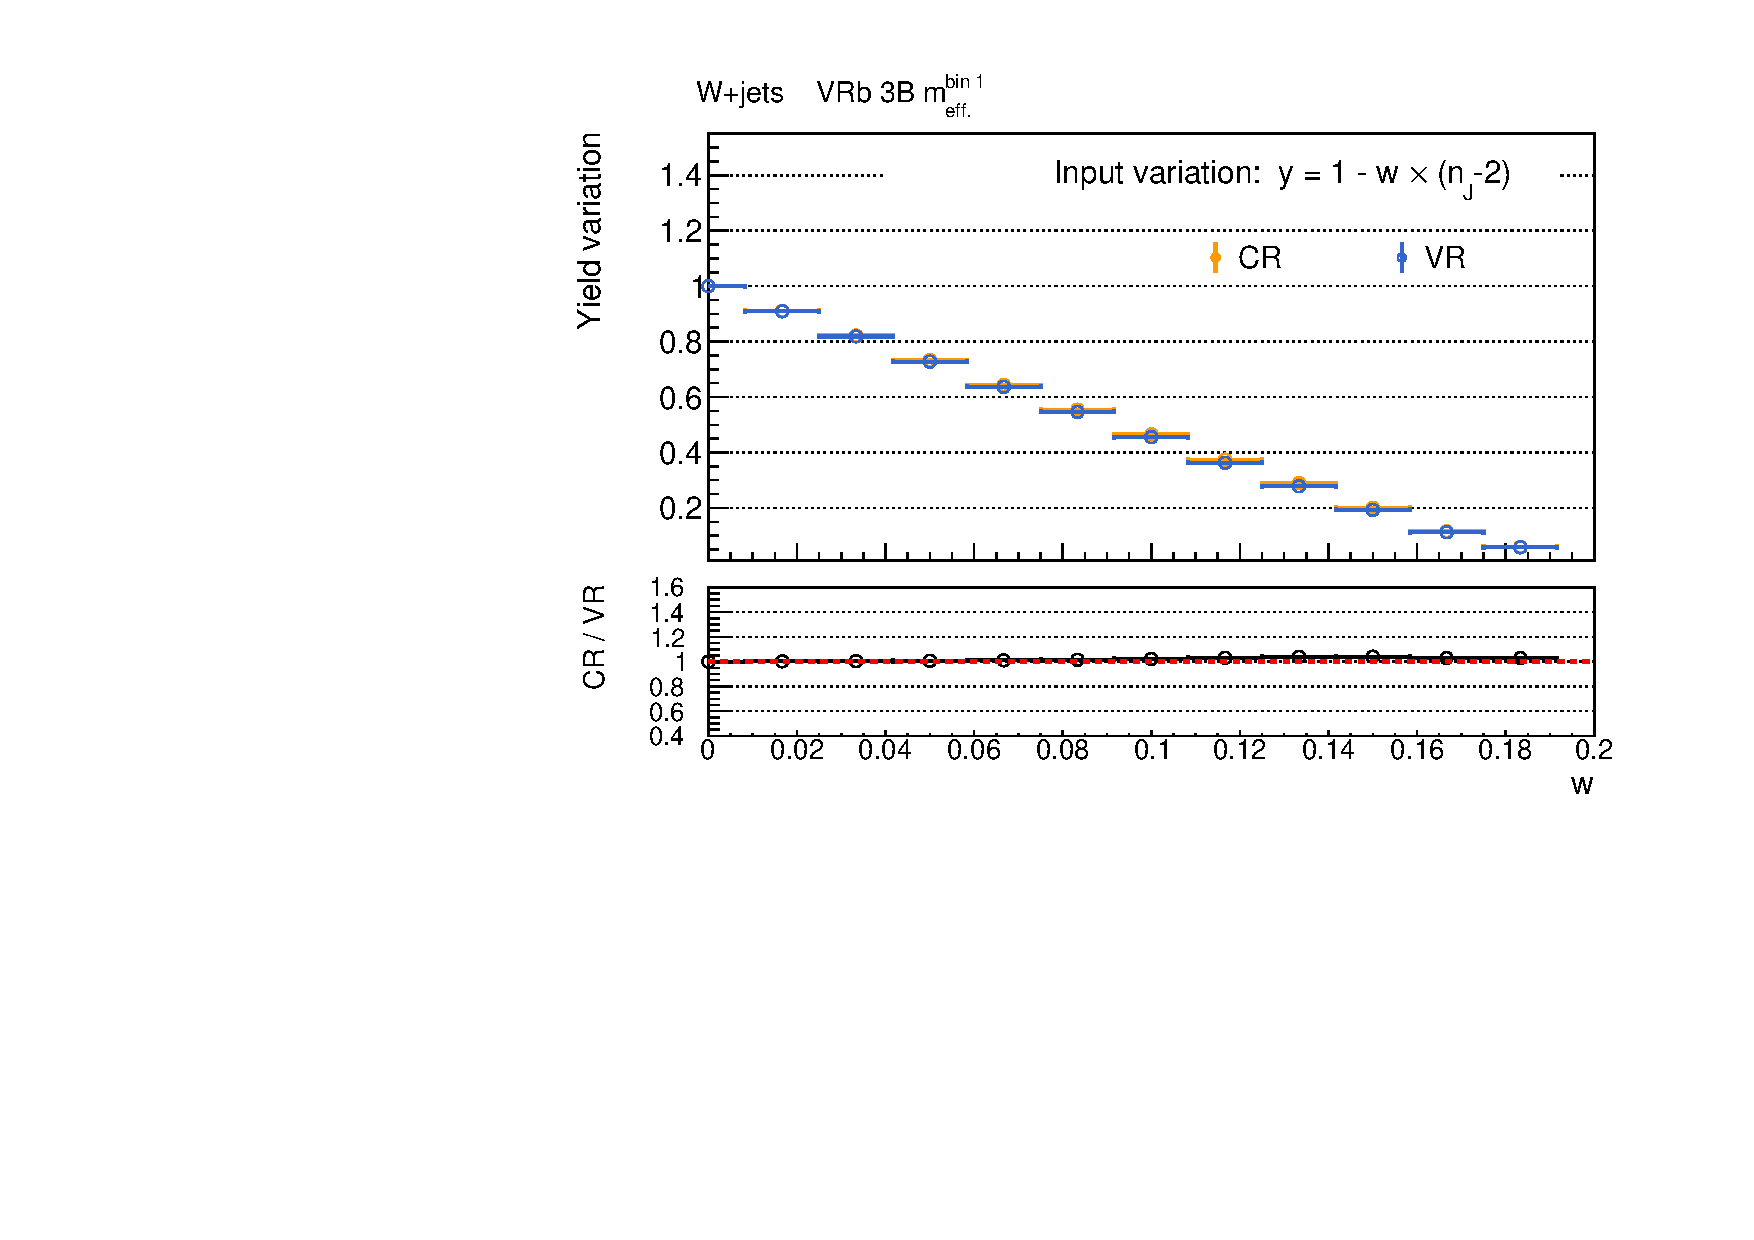
\includegraphics[width=0.488\textwidth]{figures/BGestimation/valid_extp/SFTF_wjets_VRb3BMEFF1_extp_var3B__nJet30.pdf}}
    \subfigure[]{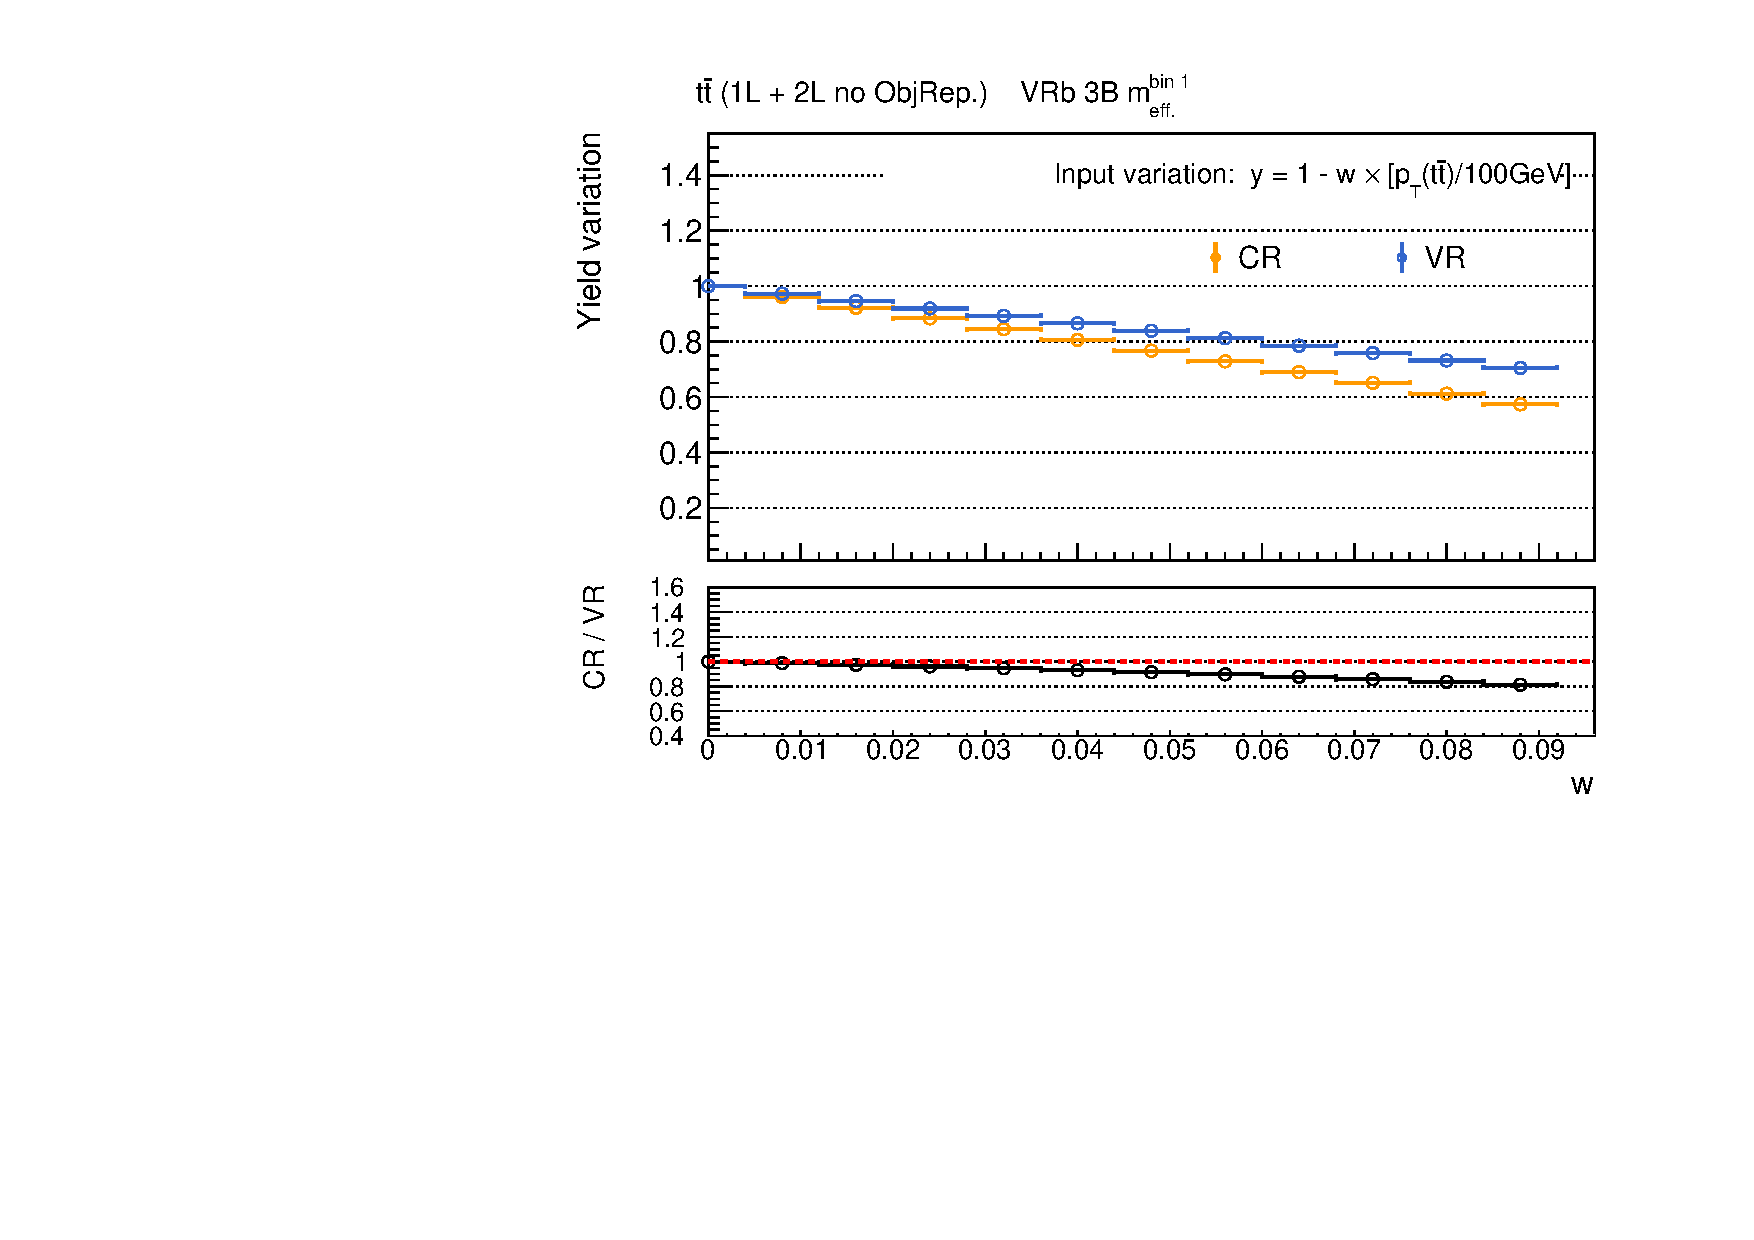
\includegraphics[width=0.488\textwidth]{figures/BGestimation/valid_extp/SFTF_ttNoObjRep_VRb3BMEFF1_extp_var3B__ttPt.pdf}}
    \subfigure[]{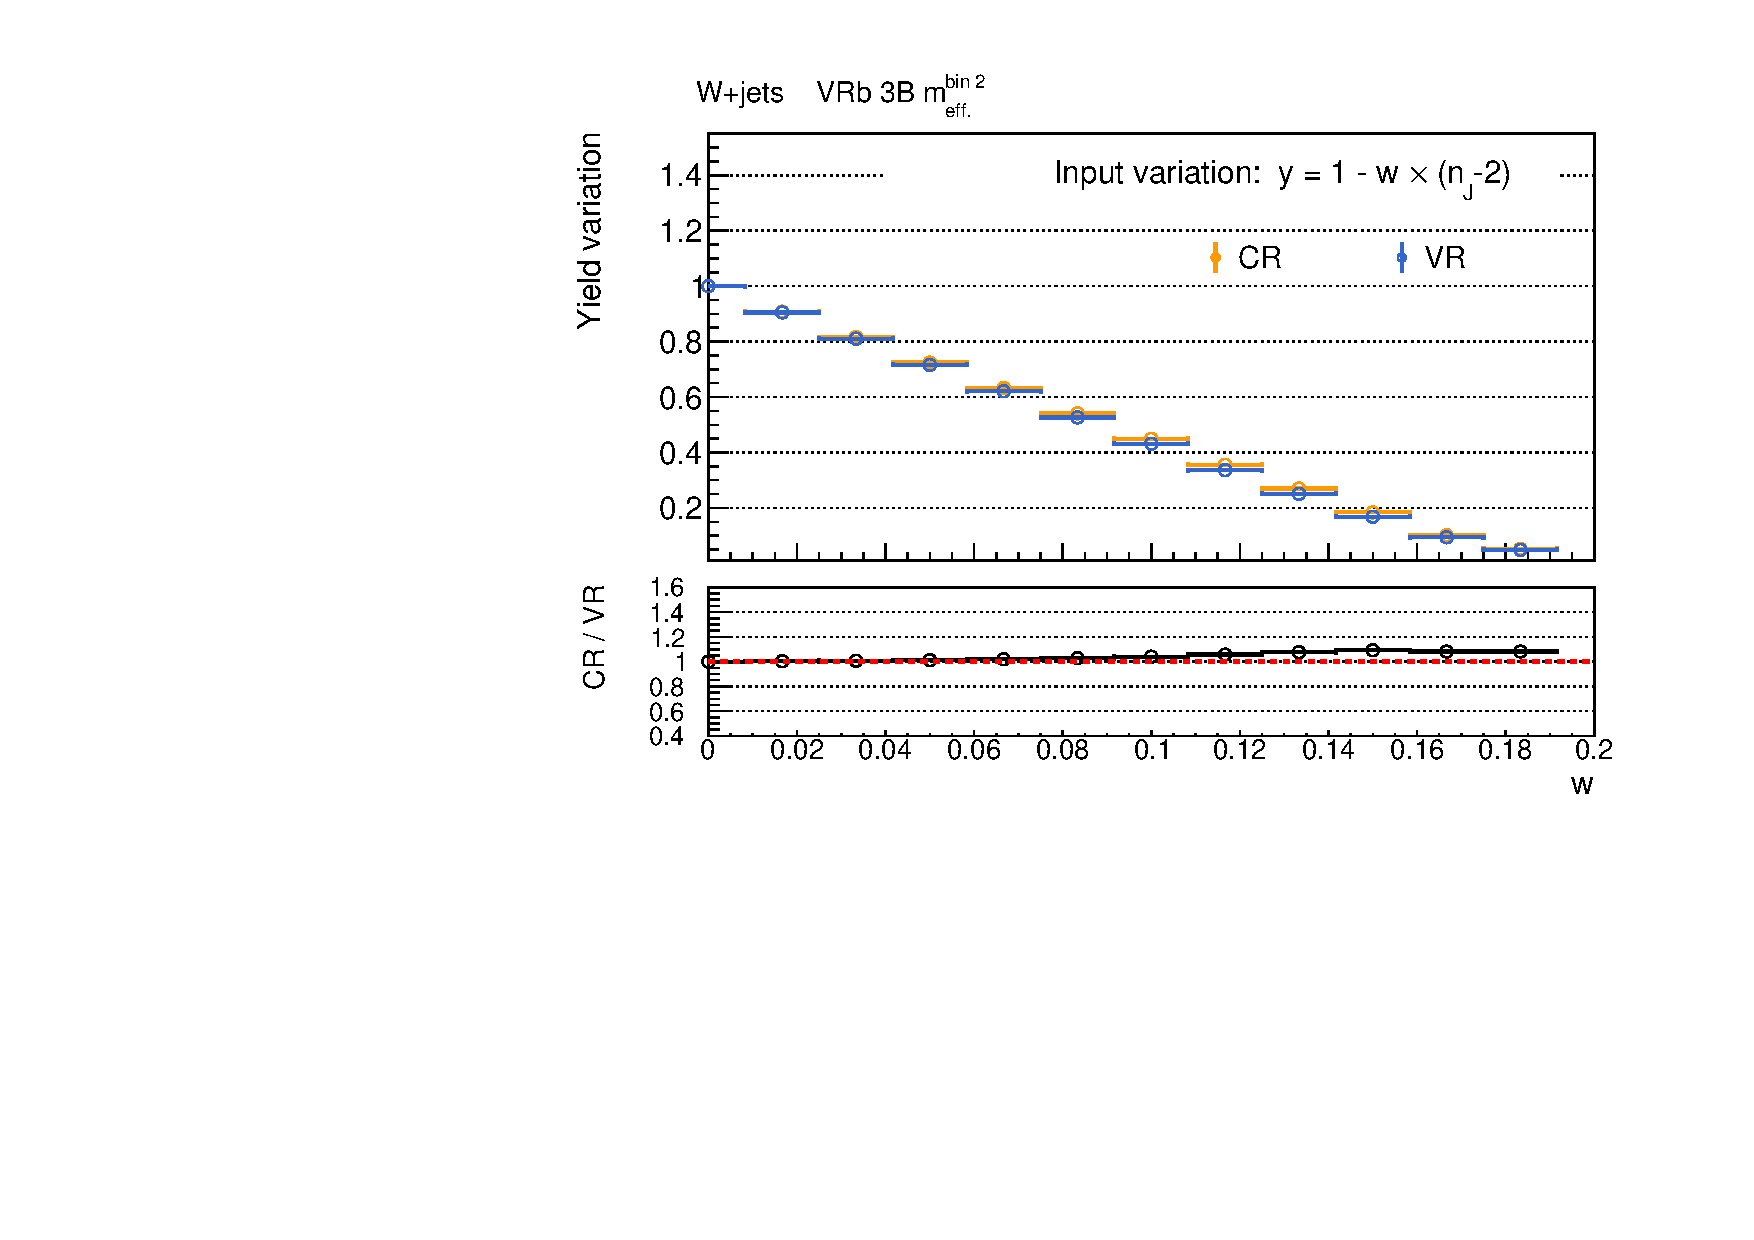
\includegraphics[width=0.488\textwidth]{figures/BGestimation/valid_extp/SFTF_wjets_VRb3BMEFF2_extp_var3B__nJet30.pdf}}
    \subfigure[]{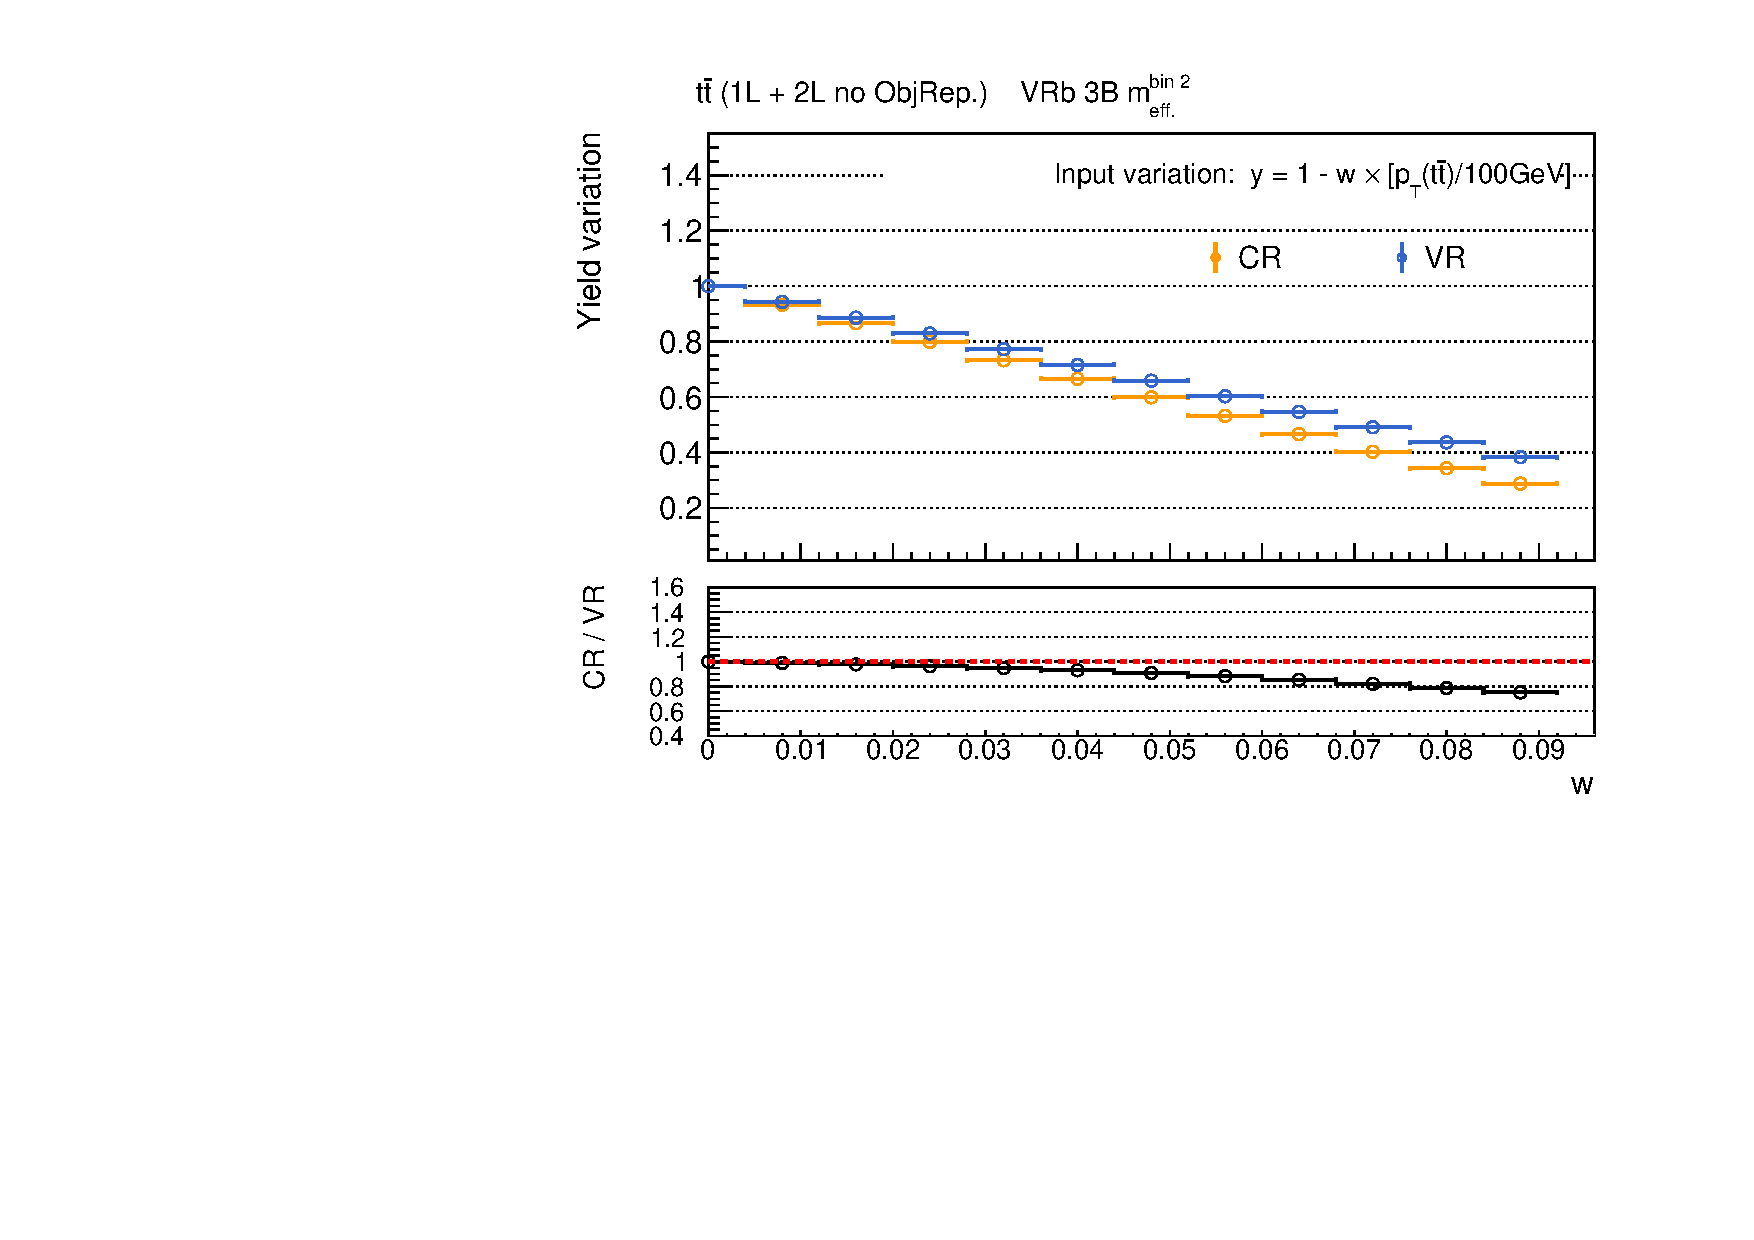
\includegraphics[width=0.488\textwidth]{figures/BGestimation/valid_extp/SFTF_ttNoObjRep_VRb3BMEFF2_extp_var3B__ttPt.pdf}}
 \caption{Extrapolation error in VRb/CR 3B. B-tagging requirement is removed for $\wjets$. Top pannels show the yield variation of $\wjets$ (left) and $\ttbar$ (right) when injecting the variation by reweighting the MC with Eq. \ref{eq::BGestimation::injected_MCvariation}. Bottom rows are the relative difference in their response against the injected variation, namely the extrapolation errir. For the $\ttbar$ process, component estimated by the object replacement method is removed.  \label{fig::BGestimation::valid_extp_VRb6J} }
\end{figure}




